\documentclass[letterpaper,12pt]{article}

% @@@@@@@@@@@@@@@@@@@@@@@@@@@@@@@@@@@@@@@@@@@@@@@@@@@@@@@@@@@@>
% VALORES A MODIFICAR POR USTED:
% @@@@@@@@@@@@@@@@@@@@@@@@@@@@@@@@@@@@@@@@@@@@@@@@@@@@@@@@@@@@>

% NOTE: Leer nota en el README sobre la font.

\newcommand{\titulo}{
Creación de algoritmo SLAM 3D para robot móvil autónomo en ambientes controlados
}
\newcommand{\ciudad}{Santiago} % e.g. Valparaíso
% TODO: Consultar el formato de los nombres:
\newcommand{\nombrealumno}{Clemente Donoso Krauss}
\newcommand{\nombreprofesor}{Erika Rosas}
\newcommand{\nombrecorreferente}{Federico Meza}
% Mes y año del examen
\newcommand{\mesexamen}{Diciembre}
\newcommand{\anioexamen}{2022}
% Dedicatoria y agradecimientos
\newcommand{\dedicatoria}{

Quiero dedicar mi memoria a mis padres Andrés y Alejandra, a mis hermanos y en especial a mi novia Paloma, quienes me brindaron su apoyo incondicional para cumplir mis sueños.
}
\newcommand{\agradecimientos}{
Me gustaría partir agradeciendo a mis hermanos Andrés, Cristián, Juan Pablo, José Tomás, Felipe e Isidora, por acompañar a este "nerd'' y de forma especial a mis padres Andrés y Alejandra, que por medio de su esfuerzo, cariño y templanza me dieron la posibilidad de seguir mis sueños, por sus ideales y enseñanzas que cada día me permiten ser un mejor ser humano. Les agradezco por no dejar de confiar en su hijo.

A mis amigos que conocí en el transcurso de estos 5 años, por que sin su ayuda, el "tatita'' no estaría acá. Gracias a todos los que permitieron de una u otra manera que hoy esté entregando mi memoria.

Agradezco también a mi profesora guía, Erika Rosas, que tomó el desafío de realizar una memoria sobre robótica conmigo. Le agradezco los consejos,las facilidades y ayuda fundamentales a la hora de escribir la memoria. Gracias por haber aceptado este gran desafío.

También gracias al "Big Boss'',  José Luis Martí por apoyarme en una de las experiencias más enriquecedoras de mi vida como lo fue la pasantía en Inria, Francia. 

Y sobretodo a mi novia Paloma, te agradezco la relación maravillosa que tenemos y también tu ayuda y amor incondicional, por ser mi faro de luz en los momentos de más tempestad, por ser mi fortaleza en los momentos en que me quería rendir, por apoyarme e impulsarme a seguir mis sueños y seguir construyendo mis robots. Esta memoria está escrita para ti y por ti, 

\newline

\textbf{GRACIAS TOTALES}
}
\newcommand{\resumen}{
Bajo el contexto de la robótica móvil la localización, navegación y percepción del entorno es una tarea fundamental, es por ello que algoritmos que engloben dichas características son esenciales.

En la memoria se propone un nuevo algoritmo SLAM 3D el cual modifica el algoritmo OctoMap existente aumentando su precisión al momento de generar rutas y generar el mapa tridimensional. El algoritmo se implementó en un robot físico y se evaluó su desempeño según su comportamiento en 5 ambientes distintos y en base a 10 métricas, dónde también se comparó su rendimiento con un algoritmo de SLAM bidimensional y  otro tridimensional.
}
\newcommand{\resumeningles}{
Under the context of mobile robotics, localization, navigation and perception of the environment it is a fundamental task, which is why algorithms that include these characteristics are essential.

In this document, a new SLAM 3D algorithm is proposed, which modifies the existing OctoMap algorithm, increasing its precision when generating routes and generating the three-dimensional map. The algorithm was implemented in a physical robot and its performance was evaluated according to its behavior in 5 different environments and based on 10 metrics, where its performance was also compared with a two-dimensional and a three-dimensional SLAM algorithm.
}
\newcommand{\palabrasclave}{
Robótica, ROS, SLAM, Navegación, Autonomía
}
\newcommand{\palabrasclaveingles}{
Robotics, ROS, SLAM, Navigation, Autonomy
}
% @@@@@@@@@@@@@@@@@@@@@@@@@@@@@@@@@@@@@@@@@@@@@@@@@@@@@@@@@@@@>

% Paquete para importar imágenes
\usepackage{graphicx}
% Directorio de las imágenes
\graphicspath{ {figures/} }

% Idioma y fuentes
\usepackage[spanish,es-tabla]{babel}
\usepackage[T1]{fontenc}
\usepackage[usenames]{color}

\usepackage{fontspec}
% Los siguientes comandos fueron sugeridos por @anibalbastiass (ver issue#5)
% para contar con Carlito en cursiva y negrita.
\setmainfont{Carlito}[BoldFont={* Bold}]
\setmainfont{Carlito}[ItalicFont={* Italic}]

% Paquete para definir cualquier tamaño de font
\usepackage{anyfontsize}

% Settear font
\setmainfont{Carlito}

% Tamaño de la página y márgenes
\usepackage[letterpaper,top=2.5cm,bottom=3cm,left=3cm,right=3cm,marginparwidth=1.75cm]{geometry}

% Determinar interlineado:
\renewcommand{\baselinestretch}{1.0}

% Eliminar sangrías:
\setlength{\parindent}{0cm}

% Paquete para definir los formatos de los títulos
\usepackage[explicit]{titlesec}

\titleformat{name=\section}[block]{\fontsize{16}{24}\selectfont\bfseries}{}{0pt}{#1}
\titleformat{name=\section,numberless}[block]{\fontsize{16}{24}\selectfont\bfseries}{}{0pt}{#1}
\titlespacing*{name=\section}{0pt}{0pt}{0.5cm}
\titlespacing*{name=\section,numberless}{0pt}{0pt}{0.5cm}

% Separación entre parrafos
\setlength{\parskip}{0.4cm}

% Paquetes de utilidad general
\usepackage{booktabs}
\usepackage[table,xcdraw]{xcolor}
\usepackage{amsmath}
\usepackage{graphicx}
\usepackage{subcaption}
\usepackage{caption}
\usepackage{float}
\usepackage[colorlinks=true, allcolors=blue]{hyperref}

\usepackage{algpseudocode}
\usepackage{amssymb}

% Formato de las tablas de contenido
% \usepackage[tocflat]{tocstyle}
\usepackage{tocstyle}
\usetocstyle{allwithdot}

% Para obtener el número de la última página
\usepackage{lastpage}

\usepackage{algorithm}
%\usepackage{algorithmic}
\usepackage{multicol}

% Header y footer
\usepackage{fancyhdr}
\fancypagestyle{portada}{
    \lhead{}
    \chead{}
    \rhead{}
    \lfoot{}
    \cfoot{\fontsize{10}{12}\selectfont \thepage}
    \rfoot{}
    \renewcommand{\headrulewidth}{0pt}
}
\fancypagestyle{intermedio}{
    \lhead{}
    \chead{\fontsize{10}{12}\selectfont\MakeUppercase{\titulo}}
    \rhead{}
    \lfoot{}
    \cfoot{\fontsize{10}{12}\selectfont Página \textbf{\thepage}\ de \textbf{\pageref{LastPage}}}
    \rfoot{}
    \renewcommand{\headrulewidth}{1pt}
}

% Comandos para secciones
\newcommand{\secnumbersection}[1]{
\addtocounter{section}{1}
\phantomsection
\section*{CAPÍTULO \thesection \texorpdfstring{\\}\ #1}
\addcontentsline{toc}{section}{CAPÍTULO \thesection : #1}
\setcounter{subsection}{0}
}
\newcommand{\secnumberlesssection}[1]{
\section*{#1}
\phantomsection
\addcontentsline{toc}{section}{#1}
\setcounter{subsection}{0}
}
\usepackage{verbatim}

\usepackage{array}
\usepackage{booktabs}

% Nombres
\addto\captionsspanish{\renewcommand{\contentsname}{ÍNDICE DE CONTENIDOS}}
\addto\captionsspanish{\renewcommand{\listfigurename}{ÍNDICE DE FIGURAS}}
\addto\captionsspanish{\renewcommand{\listtablename}{ÍNDICE DE TABLAS}}
\makeatletter
\renewenvironment{thebibliography}[1]
     {\secnumberlesssection{REFERENCIAS BIBLIOGRÁFICAS}
      \@mkboth{\MakeUppercase\bibname}{\MakeUppercase\bibname}%
      \list{\@biblabel{\@arabic\c@enumiv}}%
           {\settowidth\labelwidth{\@biblabel{#1}}%
            \leftmargin\labelwidth
            \advance\leftmargin\labelsep
            \@openbib@code
            \usecounter{enumiv}%
            \let\p@enumiv\@empty
            \renewcommand\theenumiv{\@arabic\c@enumiv}}%
      \sloppy
      \clubpenalty4000
      \@clubpenalty \clubpenalty
      \widowpenalty4000%
      \sfcode`\.\@m}
     {\def\@noitemerr
       {\@latex@warning{Empty `thebibliography' environment}}%
      \endlist}
\makeatother

% Personalizar Tabla de Contenidos

\usepackage{tocloft}
\renewcommand{\cftsecfont}{\fontsize{12}{14}\selectfont\fontspec{Carlito}}
\renewcommand{\cftsubsecfont}{\fontsize{12}{14}\selectfont\fontspec{Carlito}}
\renewcommand{\cftsubsubsecfont}{\fontsize{12}{14}\selectfont\fontspec{Carlito}}

\renewcommand\cftfigfont{\fontsize{12}{14}\selectfont\fontspec{Carlito}}

% Links sin color
\usepackage{hyperref} 
\hypersetup{ colorlinks, citecolor=black, filecolor=black, linkcolor=black, urlcolor=black }



% Comando para secciónes sin enumeración
% (sugerido por @anibalbastiass https://github.com/autopawn/tex-thesis-template/issues/5#issuecomment-916106128)
\newcommand{\secnumberlesssubsection}[1]{
\subsection*{#1}
\phantomsection
\addcontentsline{toc}{subsection}{#1}
\setcounter{subsection}{0}
}
% Forma de uso:
% \secnumberlesssubsection{"Sub seccion sin enumeración"}

% @@@@@@@@@@@@@@@@@@@@@@@@@@@@@@@@@@@@@@@@@@@@@@@@@@@@@@@@@@@@>
\begin{document}
\sloppy % Para evitar que referencias se escapen de los márgenes.

% Paquetes para algoritmos

\renewcommand{\listalgorithmname}{ÍNDICE DE ALGORITMOS}
\floatname{algorithm}{ALGORITMO}

\pagestyle{portada}
\pagenumbering{roman}
% NOTE: Este archivo contiene la portada, la dedicatoria, los agradecimientos y el resumen.
% __NO ES NECESARIO MODIFICAR ESTE ARCHIVO__, esas se modifican con los comandos que aparecen en main.tex
%@@@@@@@@@@@@@@@@@@@@@@@@@@@@@@@@@@@@@@@@@@@@@@@@@@@@@@@@@@@@@@
\begin{titlepage}
\begin{center}
\noindent
{\fontsize{18}{22}\selectfont UNIVERSIDAD TÉCNICA FEDERICO SANTA MARÍA \\}
{\fontsize{16}{19}\selectfont DEPARTAMENTO DE INFORMÁTICA \\}
{\fontsize{16}{19}\selectfont \MakeUppercase{\ciudad}\ - CHILE \\}
\vspace{1.5cm}
\includegraphics[width=4.41cm,height=3.34cm]{logo/logo.jpg} \\
\vspace{1.5cm}
{\fontsize{20}{24}\selectfont ``\MakeUppercase{\titulo}'' \\}
\vfill
{\fontsize{16}{19}\selectfont \MakeUppercase{\nombrealumno} \\}
\vfill
{\fontsize{16}{19}\selectfont MEMORIA PARA OPTAR AL TÍTULO DE \\}
{\fontsize{16}{19}\selectfont INGENIERO CIVIL EN INFORMÁTICA \\}
\vspace{1.5cm}
{\fontsize{14}{17}\selectfont Profesor Guía: \nombreprofesor \\}
{\fontsize{14}{17}\selectfont Profesor Correferente: \nombrecorreferente \\}
\vspace{2.5cm}
{\fontsize{14}{17}\selectfont \mesexamen\ - \anioexamen \\}
\end{center}
\end{titlepage}

%@@@@@@@@@@@@@@@@@@@@@@@@@@@@@@@@@@@@@@@@@@@@@@@@@@@@@@@@@@@@@@
\newpage
\setcounter{page}{2}
\
\vfill
\vfill
\begin{flushright}
\noindent {\fontsize{16}{19}\selectfont \textbf{DEDICATORIA} \\}
\end{flushright}
\begin{flushright}
\noindent 
\dedicatoria
\end{flushright}
\vfill
%@@@@@@@@@@@@@@@@@@@@@@@@@@@@@@@@@@@@@@@@@@@@@@@@@@@@@@@@@@@@@@
\newpage
\begin{center}
\noindent {\fontsize{16}{19}\selectfont \textbf{AGRADECIMIENTOS} \\}
\end{center}
\noindent 
\agradecimientos
\vfill
%@@@@@@@@@@@@@@@@@@@@@@@@@@@@@@@@@@@@@@@@@@@@@@@@@@@@@@@@@@@@@@
\newpage
\secnumberlesssection{RESUMEN}
\vspace{0.3cm}
\noindent \textbf{Resumen---}
\resumen 
\ \\
\vspace{0.3cm} \\
\noindent \textbf{Palabras Clave---}
\palabrasclave 
\ \\
% @@@@@
\vspace{1.2cm} \\
% @@@@@
%\noindent {\fontsize{16}{19}\selectfont \textbf{ABSTRACT}}
%\vspace{1.2cm} \\
\secnumberlesssection{ABSTRACT}
\vspace{0.3cm}
\noindent \textbf{\emph{Abstract}---}
\resumeningles 
\ \\
\vspace{0.3cm} \\
\noindent \textbf{\emph{Keywords}---}
\palabrasclaveingles
\ \\
%@@@@@@@@@@@@@@@@@@@@@@@@@@@@@@@@@@@@@@@@@@@@@@@@@@@@@@@@@@@@@@


\newpage
\secnumberlesssection{GLOSARIO}

{\setlength{\parskip}{0cm} % Para evitar saltar entre cada elemento nombrado.
%Colocar aquí siglas:

CONICYT:Comisión Nacional de Investigación Ciencia y Tecnología

DI: Departamento de Informática.

EFK: Extended Kalman Filter

GPS: Global Positioning System

IMU: Inertial Measurement Unit

LIDAR: Laser Imaging Detection and Ranging

MCL: Monte Carlo Localization

NASA: National Aeronautics and Space Administration

ROS: Robot Operating System

RGB: Red, Green and Blue

SLAM: Simulatenous Localization and Mapping

TCP: Transmission Control Protocol

TF: Transformation Frames

URDF: Unified Robot Description Format

UTFSM: Universidad Técnica Federico Santa María.

XML: Extensible Markip Language

}



%Índice de contenidos:
\newpage
\thispagestyle{portada}
\tableofcontents



%Índice de figuras:
\newpage
\thispagestyle{portada}
\phantomsection
\addcontentsline{toc}{section}{ÍNDICE DE FIGURAS}
\listoffigures

\phantomsection
\addcontentsline{toc}{section}{ÍNDICE DE TABLAS}
\listoftables



\phantomsection
\addcontentsline{toc}{section}{ÍNDICE DE ALGORITMOS}
\listofalgorithms

\newpage
\pagestyle{intermedio}
\pagenumbering{arabic}
\secnumberlesssection{INTRODUCCIÓN}

Los algoritmos de navegación y localización simultánea en la robótica son relativamente nuevos, sin embargo en las últimas dos décadas dado los avances de la tecnología, grandes avances se han producido en el área de la robótica móvil permitiendo algoritmos más avanzados y optimizados.

En la actualidad, existen diversos sensores y algoritmos para enfrentar el problema de la localización de un robot, es por ello que es esencial darle solución a los 4 problemas principales de dichos algoritmos: La asociación de los datos, la incertidumbre, el error acumulativo y la complejidad temporal. Para darle solución a dicho problema en el documento se plantea la implementación de un algoritmo SLAM 3D que permita generar el mapa tridimensional y bidimensional del entorno utilizando una cámara de profundidad y un LIDAR y de esta manera mejorar la asociación de los datos y por ende, generar mapas más precisos a un bajo coste monetario.

El objetivo del documento es la creación de un algoritmo de localización y navegación simultánea, el cual se busca cumplir a través de la investigación del estado de arte de dichos algoritmos, el diseño propiamente tal de dicho algoritmo utilizando solo una cámara de profundidad y un LIDAR y también la implementación del algoritmo en un robot físico y así evaluar en ambientes controlados y reales el desempeño de este.

La estructura del documento presenta 6 capítulos: El capítulo 1 corresponde a la definición del problema en donde se explica el contexto, el objetivo y los impactos de darle solución a la problemática del SLAM en la robótica. Luego en el capítulo 2 se presenta el marco conceptual para entregar los conocimientos técnicos al lector así como también, se describe el estado del arte de los algoritmos SLAM. En el capítulo 3 se plantea la propuesta de solución, en donde se describe el punto de partida y luego el diseño del algoritmo. Luego, en el capítulo 4 se realiza el diseño experimental de la memoria en donde se describe el robot utilizado para la memoria y también se detallan tanto las métricas de evaluación como los 5 ambientes experimentales utilizados. Posteriormente, en el capítulo 5 se detallan los resultados obtenidos en los 5 ambientes, así como también se describe el proceso de calibración de los sensores. Finalmente, en el capítulo 6 se realizan las conclusiones de la memoria y se plantea los lineamientos para un trabajo futuro a quienes deseen continuar con la investigación.

\begin{comment}
Debe proporcionar a un lector los antecedentes suficientes para poder contextualizar en general la situación tratada, a través de una descripción breve del área de trabajo y del tema particular abordado, siendo bueno especificar la naturaleza y alcance del problema; así como describir el tipo de propuesta de solución que se realiza, esbozar la metodología a ser empleada e introducir a la estructura del documento mismo de la memoria.

En el fondo, que el lector al leer la Introducción pueda tener una síntesis de cómo fue desarrollada la memoria, a diferencia del Resumen dónde se explicita más qué se hizo, no cómo se hizo.

\end{comment}

\newpage
\secnumbersection{DEFINICIÓN DEL PROBLEMA}

\subsection{CONTEXTO}
La industria de la robótica crece año tras año y junto con esto, la inversión en crear nuevos robots que satisfagan las necesidades humanas. El estudio realizado por \cite{graetz_online_nodate} entregó que la aplicación de robots en la industria habría implicado una mejora de 2.36 \% en la productividad anual entre los años 1993 y 2007. Lo anterior es demostración clara que la utilización de robots no solo en la industria, sino en los hogares, centros educativos y zonas públicas se debe incentivar, y como desafío se deben crear robots adaptables a dichos entornos. Dentro del área podemos encontrar diversos tipos de robots según su aplicación como lo son los robots industriales, los de servicio, los médicos y otras áreas más nuevas como los robots suaves, los cuales están compuestos por estructuras flexibles que con diferencias de presión de aire logran el movimiento (a diferencia de los robots rígidos, los cuales utilizan actuadores o motores para lograr dicho robot), los robots submarinos, los cuales operan en el mundo acuático para el estudio de la vida marina, fondo marino y otras áreas más .Sin embargo, los robots se pueden separar dentro de 2 grandes grupos, los robots estáticos y los robots móviles \cite{thrun_probabilistic_2005}.

Los robots estáticos fueron los pioneros en el área de la robótica y como dice su nombre, se encuentran fijos a la superficie, por lo que el lugar en donde este se implemente, debe adaptarse a la posición del robot, esto genera dificultades a posibles cambios que se requieran en el lugar de trabajo debido a los altos costos asociados, ya que se debe desmontar el robot y crear una nueva zona de trabajo para este. Por otro lado, los robots móviles, se pueden encontrar montados en una plataforma móvil, disponer de ruedas o extremidades para desplazarse, lo que les da mayores funcionalidades y más capacidades que los primeros, sin embargo, la implementación de estos sugiere un estudio avanzado de la robótica y como los robots perciben el entorno, por lo que hace más difícil su estudio \cite{fahimi_autonomous_2009}.

Debido a las oportunidades de estudio que se pueden encontrar en el área de la robótica móvil, la escalabilidad de los proyectos y los desafíos presentes que se requieren resolver, la memoria se centrará en dicha área. Los desafíos que se puedan encontrar son múltiples, siendo el más importante, el de la navegación y localización de un robot dentro de un entorno \cite{noauthor_global_nodate}. En el área de robótica móvil el desafío principal que se debe tener en cuenta es el ``cómo'' el robot logra entender el entorno y también ``cómo'' logra a través de sensores y/o cámaras posicionarse en este, ya que esto es clave para que el robot pueda cumplir de manera correcta la tarea para la cual fue creado \cite{quigley_programming_nodate}. Debido a lo anterior, es esencial plantear algoritmos correctos y adaptable a las necesidades que se tengan.

\subsubsection{ÁRBOL DEL PROBLEMA}

El árbol del problema definida para encapsular la memoria se puede observar en la figura \ref{fig:arbol_del_problema}, de dónde se extraen los objetivos que se pueden observar en la sección de objetivos.
\begin{figure}[h]
\centering
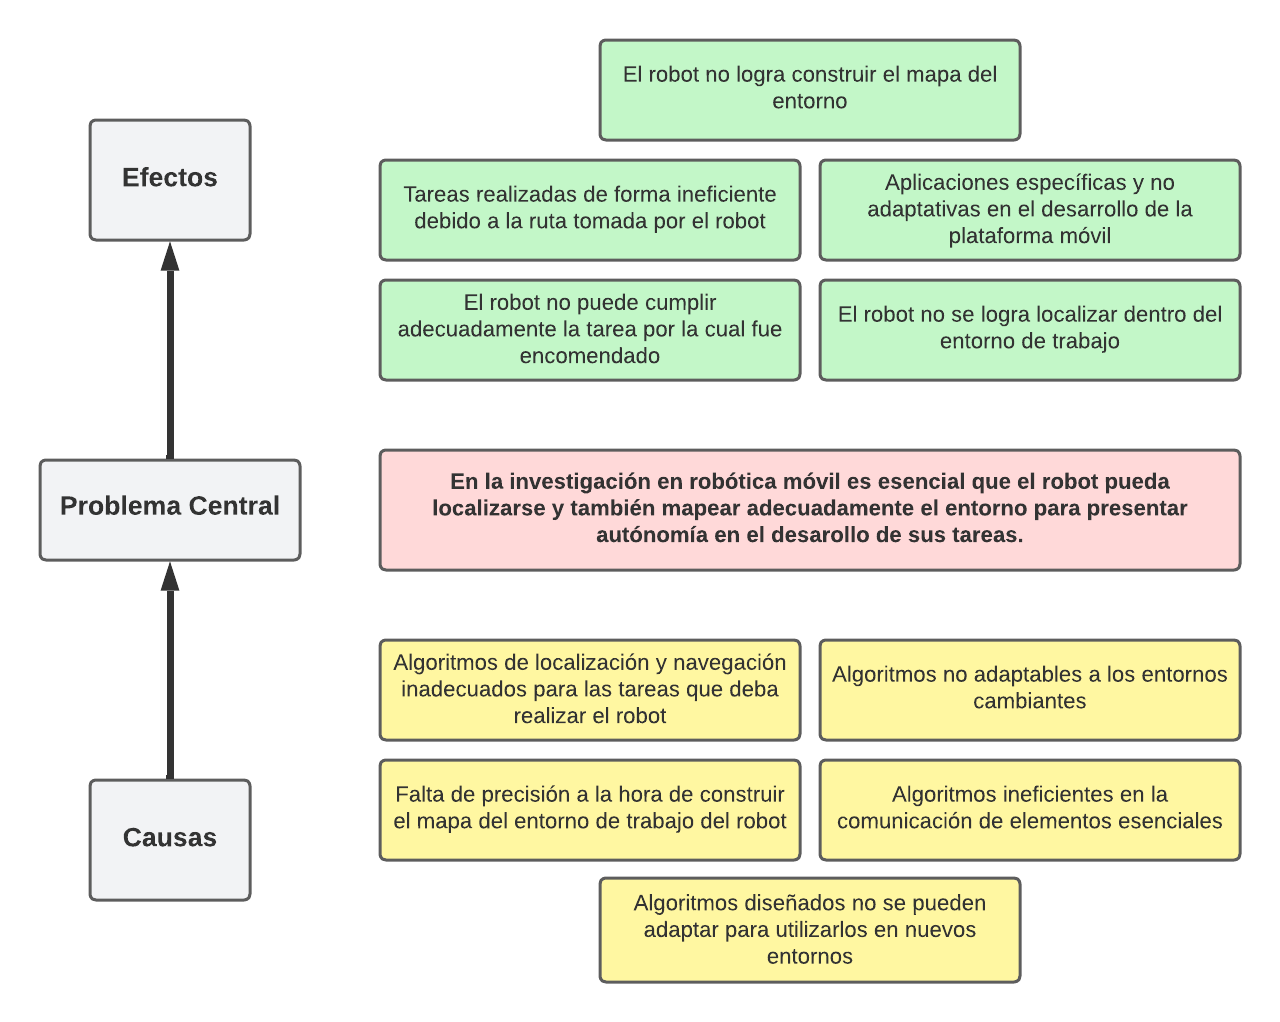
\includegraphics[width=1\textwidth]{figures/01definicion_problema/arbol_del_problema.png}
\caption{\label{fig:arbol_del_problema} Árbol del Problema} Fuente: Fabricación propia
\end{figure}

\subsubsection{SITUACIÓN EN CHILE}

La investigación en robótica en Chile es deficiente y poco desarrollada. Existen menos de una decena de laboratorios de robótica capacitados para la construcción e investigación profesional en el área. Con todo, es importante destacar que existen diversas necesidades que requieren ser satisfechas por la robótica y diversos escenarios o ambientes para poner a prueba los robots. Por otra parte se estima que durante la próxima década cerca del 70\% de la población chilena se encontrará en contacto con algún robot \footnote{A partir del 2018 CONICYT incentiva la investigación en el área de la robótica dando prioridad a los becados interesados en dicha área https://www.conicyt.cl/becasconicyt/2018/03/28/magister-becas-chile-2018-abre-convocatoria-en-areas-de-interes-prioritario/ }. Existen diversos campos de aplicación de esta área, tales como: En la minería analizando y apoyando las labores, en hospitales llevando insumo a las habitaciones, en nuestros hogares cuidándolos mientras no estamos, entre otras más. 

Los campos anteriormente mencionados, tienen como denominador común que el robot para suplir la tarea debe mapear el entorno para luego localizarse y planificar una ruta para realizar la tarea para la cual fue asignado. Bajo esta lógica, es de suma importancia tener algoritmos adaptables a los cambios en el entorno. Por otra parte, se puede observar que la diversidad natural de Chile plantea diversos escenarios que no solo pondrán a prueba los robots a las inclemencias del tiempo, sino también, verificar los algoritmos y el comportamiento de la máquina antes estos escenarios, tal cual como lo ha hecho la \textit{National Aeronautics and Space Administration} con sus \textit{rovers} \cite{wei_autonomous_2015}.

\newpage
\subsection{OBJETIVOS}

El objetivo general de esta memoria consiste en \textit{crear un algoritmo de localización y navegación simultánea utilizando una cámara de profundidad y un lidar para un robot móvil autónomo en ambientes controlados.
}

\subsubsection{OBJETIVOS ESPECÍFICOS}
Para poder cumplir con el objetivo general previamente mencionado, es necesario realizar los siguientes objetivos específicos:
\begin{enumerate}
    \item Analizar los algoritmos de localización y navegación simultánea para adquirir los conocimientos del área a través de una investigación del estado del arte.
    
    \item Diseñar un algoritmo de localización y navegación simultánea tridimensional por medio de la utilización de una cámara de profundidad y un lidar para construir un mapa tridimensional de bajo costo.
    
    \item Evaluar el desempeño del algoritmo propuesto por medio de la implementación física del robot considerando diversos ambientes de pruebas.
\end{enumerate}

\newpage
\subsection{IMPACTO DE SOLUCIONAR EL PROBLEMA}

La investigación en robótica no es algo trivial, pero si es esencial en los tiempos actuales y más aún en los tiempos que se avecinan donde la robótica será un pilar fundamental en la sociedad \cite{rivera_taiba_efectos_2019}. La robótica implica la colaboración de múltiples áreas como lo es la electrónica, la informática y la mecánica, cada una con sus desafíos e implicancia, los cuales deben ser resueltos de manera individual para la creación de un robot. Es por ello, que la metodología de investigación debe ser estructurada y seguir los lineamientos planteados por la comunidad internacional de robótica.

Desde el punto de vista de la informática, uno de los problemas esenciales en la robótica móvil es la navegación, localización y mapeo de un robot en un entorno, siendo aún más complejo dicho desafío en entornos no controlados \cite{fahimi_autonomous_2009}. Ésta es una problemática que requiere ser estudiada y analizada al momento de diseñar un robot móvil autónomo, ya que la movilidad, localización y mapeo son la piedra angular de todo robot autónomo. 

Actualmente, existen una diversidad de algoritmos de localización y navegación simultánea, los cuales tienen requerimientos específicos y están diseñados para suplir necesidades específicas. Estos algoritmos están fuertemente apoyados tanto en los sensores que utilizan los robots, como también en los cambios existentes en el ambiente \cite{omara_indoor_2015}. Por lo que es de suma importancia evaluar el comportamiento de dichos algoritmos y su adaptabilidad a los cambios en el entorno y de esta manera implementar algoritmos de manera eficiente según el ambiente y el requerimiento que se requiere satisfacer.

Es por ello que un análisis exhaustivo a los principales algoritmos de localización y navegación simultánea, evaluar el comportamiento en diversos ambientes a través de distintas métricas estandarizadas por la comunidad mundial y valuar cumplimiento de los requerimientos es de suma importancia en la investigación en robótica \cite{anis_koubaa_robot_2016} y sobretodo, darle solución a las problemáticas esenciales de la técnica (definidas en el estado del arte), ya que de esta manera, además de incentivar la creación de plataformas autónomas móviles para el estudio del área, el análisis permitirá destinar de mejor manera los recursos asociados a la investigación y a su vez, generar una relación entre los requerimientos del sistema y los algoritmos evaluados.

\subsubsection{METODOLOGÍA DE INVESTIGACIÓN}
Tal como se nombró en la sección anterior, la metodología a utilizar debe seguir los lineamientos verificados y comprobados por la comunidad internacional de robótica, ya que de esta manera, se disminuyen los riesgos de quemar componentes, se disminuyen los riesgos de posibles errores estructurales y en casos más graves, poner en riesgo la vida humana. Si bien existen varios puntos de vista sobre la manera más adecuada para la investigación en robótica, la metodología que se utilizará para llevar a cabo la memoria será una de las descritas por \cite{inves_2004}, \textit{`` la metodología del ciclo de vida de Buchanan''}.

El ciclo de vida de Buchanan presenta la estructura que se puede observar en la Figura \ref{fig:Buchanan},
\begin{figure}[h]
    \centering
    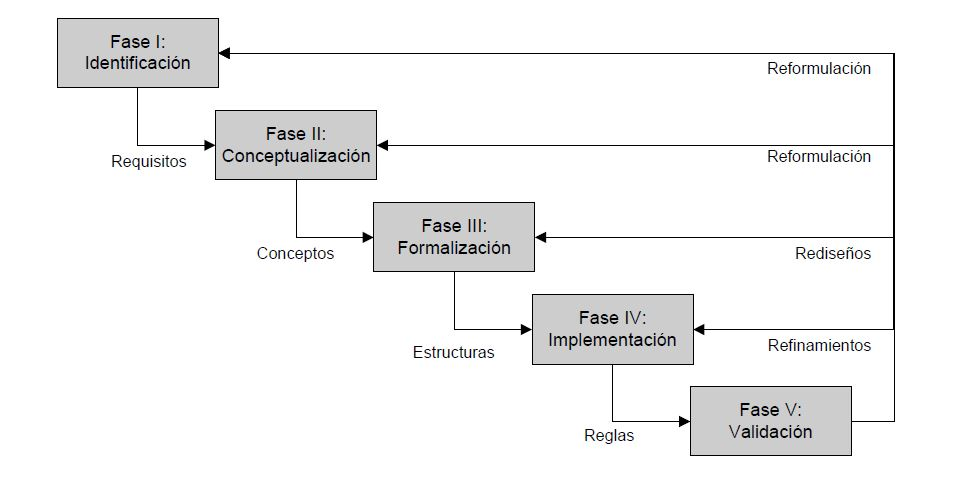
\includegraphics[width=0.8\textwidth]{figures/01definicion_problema/metodologia_Bu.JPG}
    \caption{\label{fig:Buchanan} Metodología del Ciclo de vida de Buchanan} 
    Fuente: \cite{buchanan_2000}
\end{figure}
ya que, producto de los alcances de la memoria y los objetivos planteados es la más adecuada para realizarla. Esta metodología comprende las siguientes fases durante la investigación:
\begin{itemize}
    \item \textbf{Identificación: }Corresponde a la fase inicial en la cual se investiga sobre el estado del arte de la memoria, investigaciones realizadas y sobretodo está centrada en la adquisición de los conocimientos mínimos para la realización de la memoria, en este caso, la investigación del estado del arte de la robótica móvil, investigación sobre el framework ROS e investigar sobre la navegación autónoma. De esta manera se limita los alcances y se determina como se enfrentará al problema de la navegación autónoma.
    \item \textbf{Conceptualización: }Corresponde a la continuación de la fase anteriormente descrita en donde se definen los problemas en concretos que se deben resolver, de esta manera, se definen los conceptos más relevantes que deben ser tratados en la memoria, como por ejemplo, los conceptos de localización y navegación en la robótica móvil autónoma. También se deben reconocer las estrategias que se utilizarán para dar solución al problema.
    \item \textbf{Formalización: }Una vez que se construye el marco teórico, en la fase de la formalización, se dará pie a organizar la información recaba y los conocimientos adquiridos para dar pie a la realización del primer prototipo (diseño) que da solución al problema o los problemas identificados en las fases anteriores.
    \item \textbf{Implementación: }Corresponde a la fase dónde se implementa propiamente tal el prototipo diseñado en la fase anterior, es una fase iterativa dónde se ajustan los parámetros, se implementan los diversos algoritmos investigados y se realizan las diversas estrategias planteadas anteriormente. 
    \item \textbf{Validación: }La última fase corresponde a la fase de validación en dónde, el prototipo se validará frente a diversas situaciones y ambientes, de esta manera se corroborará que la investigación fue la adecuada para resolver los objetivos descritos.
\end{itemize}




\newpage
\secnumbersection{MARCO CONCEPTUAL}

En el presente capítulo, se detallarán los conceptos fundamentales que son requeridos tanto para el desarrollo de la memoria, como también para el entendimiento de esta. Son definidos los conceptos como el framework \textit{robot operating system}, la robótica, los algoritmos de localización, mapeo y navegación y los ambientes de simulación gazebo y rviz.

\subsection{ROBÓTICA}
La concepción de la idea de una máquina que ayude al ser humano proviene del siglo 3 antes de Cristo, donde se concibe la primera idea de una máquina mecánica que esté creada con la única utilidad en ayudar al ser humano en sus actividades diarias. Sin embargo, la concepción moderna de robots proviene de la edad media con los autómatas de Da Vinci y Al Jazari, los cuales se consideran los primeros robots.
La robótica moderna es un área multidisciplinaria de la ingeniería en donde conjuntamente trabajan las ingenierías electrónica, mecánica, informática para el estudio, análisis, diseño y creación de máquinas autónomas capaces de realizar tareas asignadas o aprender mediante las realizan, tal y como lo muestra la Figura \ref{fig:areas_robotica}. 
\begin{figure}[h]
\centering
\includegraphics[width=0.5\textwidth]{figures/02marco_conceptual/robótica.png}
\caption{\label{fig:areas_robotica} Áreas de la Robótica} 
Fuente: \cite{area_rob_2017}
\end{figure}

\newpage
\subsection{ROBOT OPERATING SYSTEM}
\textit{Robot Operating System} (ROS) es un \textit{framework} orientado a la investigación en robótica. Si bien ROS no es un sistema operativo, provee de los servicios estándar de uno como el control de dispositivos de bajo nivel, la implementación de funcionalidad de uso común, abstracción de hardware, el envío de mensajes entre procesos, entre otros elementos. Está basado en una arquitectura de grafos en donde cada nodo implementa una funcionalidad específica, estos pueden recibir o enviar mensajes, controlar actuadores o sensores, comunicarse con otros nodos, entre otras funcionalidades.
ROS está compuesto por 3 conceptos esenciales que se nombraron anteriormente:
\begin{itemize}
    \item \textbf{Nodos: } Corresponden a los archivos ejecutables que utilizará ROS para realizar acciones. Los nodos se podrán comunicar con otros nodos mediante canales establecidos y el paso de mensajes estructurados.
    \item \textbf{Canales: } Corresponden a los diversos paradigmas de comunicación que se detallarán en la siguiente sección, mediante los cuales los nodos enviarán mensajes.
    \item \textbf{Mensajes: } Corresponden a datos estructurados mediante una cabecera y campos específicos, tales como enteros, flotantes, textos, entre otros.
\end{itemize}

\subsubsection{PARADIGMAS DE COMUNICACIÓN}
Para realizar la comunicación entre los nodos, ROS presenta 3 tipos de paradigmas de comunicación los cuales utilizan los protocolos TCP y UDP (TCPROS y UDPROS respectivamente) para realizar el intercambio de mensajes, tal como lo detalla Anis Koubaa en su libro \cite{anis_koubaa_robot_2016}.

\begin{itemize}
    \item \textbf{Topics: } El paradigma de comunicación \textit{Publisher - Subscriber} se presenta cuando uno de los nodos de ROS está publicando o está suscrito a un tópico el cual contiene un mensaje determinado, dicho mensaje está definido por un nombre y su contenido. Este, se envía por un tópico específico creando un canal de comunicación entre los nodos que lo necesiten. Esta comunicación se realiza solo en una dirección y se puede dar comunicación 1* a 1* \footnote{Soporta la comunicación 1 a 1, 1 a muchos y también muchos a 1}. Esta comunicación se puede ver descrita en la Figura \ref{fig:ROS_topics}.
    \begin{figure}[h]
    \centering
    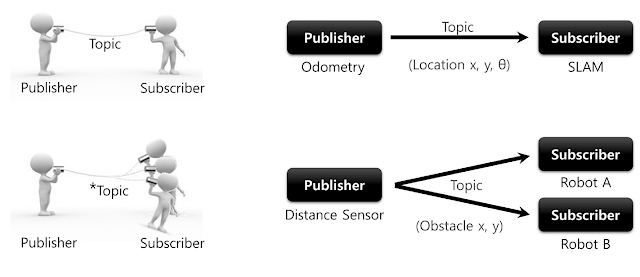
\includegraphics[width=0.7\textwidth]{figures/02marco_conceptual/ROS_topic.png}
    \caption{\label{fig:ROS_topics} Paradigma de comunicación - Topics} 
    Fuente: \cite{robin_robotics_2019}
    \end{figure}
    
    \item \textbf{Server Services: }
    El paradigma de comunicación \textit{Server Services} se plantea la utilización de un servidor donde el cliente envía una petición al servidor y el servidor le entrega una respuesta. Este paradigma de comunicación es síncrono, por lo que el cliente quedará esperando la respuesta del servidor y también es bidireccional a diferencia del anterior. Esta comunicación se puede ver descrita en la Figura \ref{fig:ROS_services}.
    
    \begin{figure}[h]
    \centering
    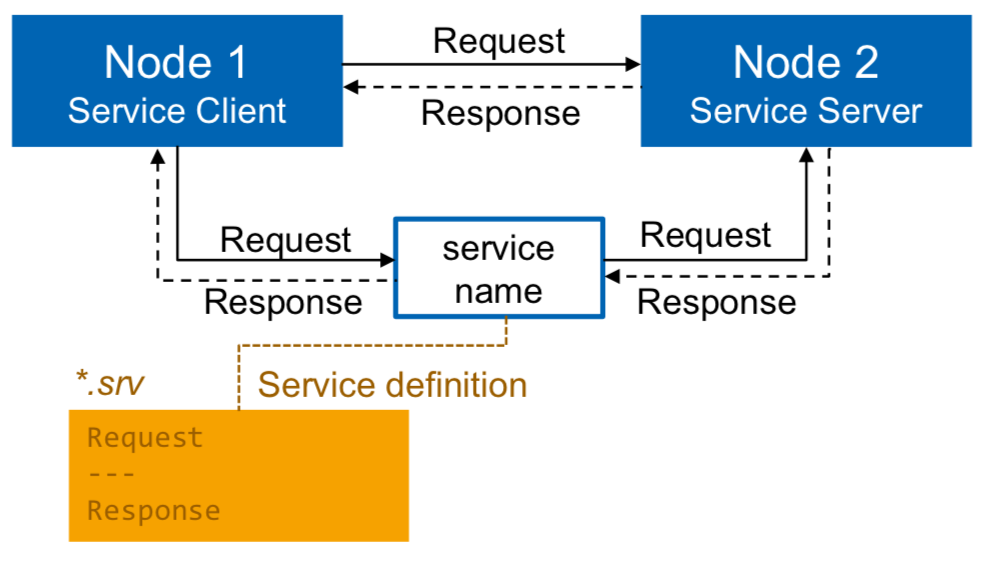
\includegraphics[width=0.7\textwidth]{figures/02marco_conceptual/ROS_service.png}
    \caption{\label{fig:ROS_services} Paradigma de comunicación - Server Services} 
    Fuente: \cite{ros_services_2018}
    \end{figure}
    
    \item \textbf{Server Actions: }
    El paradigma de comunicación \textit{Server Actions} al igual que el paradigma descrito anteriormente, plantea la utilización de un servidor donde el cliente envía una petición al servidor y el servidor le entrega una respuesta, sin embargo, esta vez la comunicación es asíncrona, por lo que el cliente puede seguir realizando sus tareas sin esperar la respuesta del servidor. Esta comunicación se puede ver descrita en la Figura \ref{fig:ROS_actions}.
    
    \begin{figure}[h]
    \centering
    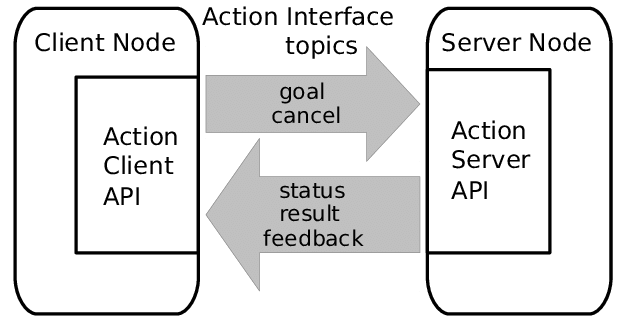
\includegraphics[width=0.7\textwidth]{figures/02marco_conceptual/ROS_action.png}
    \caption{\label{fig:ROS_actions} Paradigma de comunicación: Server Actions} 
    Fuente: \cite{andres_rosoclingo_2013} 
    \end{figure}
    \end{itemize}
    
    Cada uno de estos paradigmas de comunicación se utilizarán en el robot para enviar mensajes entre los actuadores y el procesador principal, para enviar la imagen que se está observando al computador, para controlar el robot, enviar coordenadas, observar el mapa que se está creando, la ruta definida, entre otras tareas y análisis que se realizarán.

\newpage
\subsection{SIMULACIÓN}
La simulación es un elemento no menor en el área de la robótica, ya que permite testear de manera segura los robots diseñados, permite utilizar los algoritmos creados, analizar el comportamiento del robot sin comprometer su estructura física y verificar los posibles errores que se pueda observar. Dentro del estado del arte de la robótica móvil, los dos motores gráficos que se utilizan por excelencia son \textit{Gazebo} y \textit{RVIZ}. Takaya presenta una aproximación sobre como simular entornos y probar robots utilizando Gazebo \cite{takaya_simulation_2016} y las bases necesarias para testear algoritmos de localización y navegación en entornos controlados.

\subsubsection{GAZEBO}
Gazebo es un  software de \textit{open source} diseñado para simplificar el desarrollo de robots y aplicaciones de alto rendimiento. Está basado en la arquitectura \textit{cliente/servidor}. Se presenta esta arquitectura como la comunicación de dos actores, el cliente el cual consume los recursos y el servidor el cual provee dichos recursos \cite{lizama_redes_nodate}. Gazebo es considerado el simular más importante en la industria de la robótica, donde se pueden simular entornos complejos, físicas realísticas para una mayor semejanza con las aplicaciones reales del robot y estructuras complejas como se muestra en la Figura \ref{fig:ROS_gazebo}. Es esencialmente usado en el área de la investigación cuando no se dispone físicamente del robot y se requiere testear los algoritmos creados o el comportamiento del robot, por lo que se simula el entorno real y lo que el robot está efectivamente viendo.


\begin{figure}[h]
    \centering
    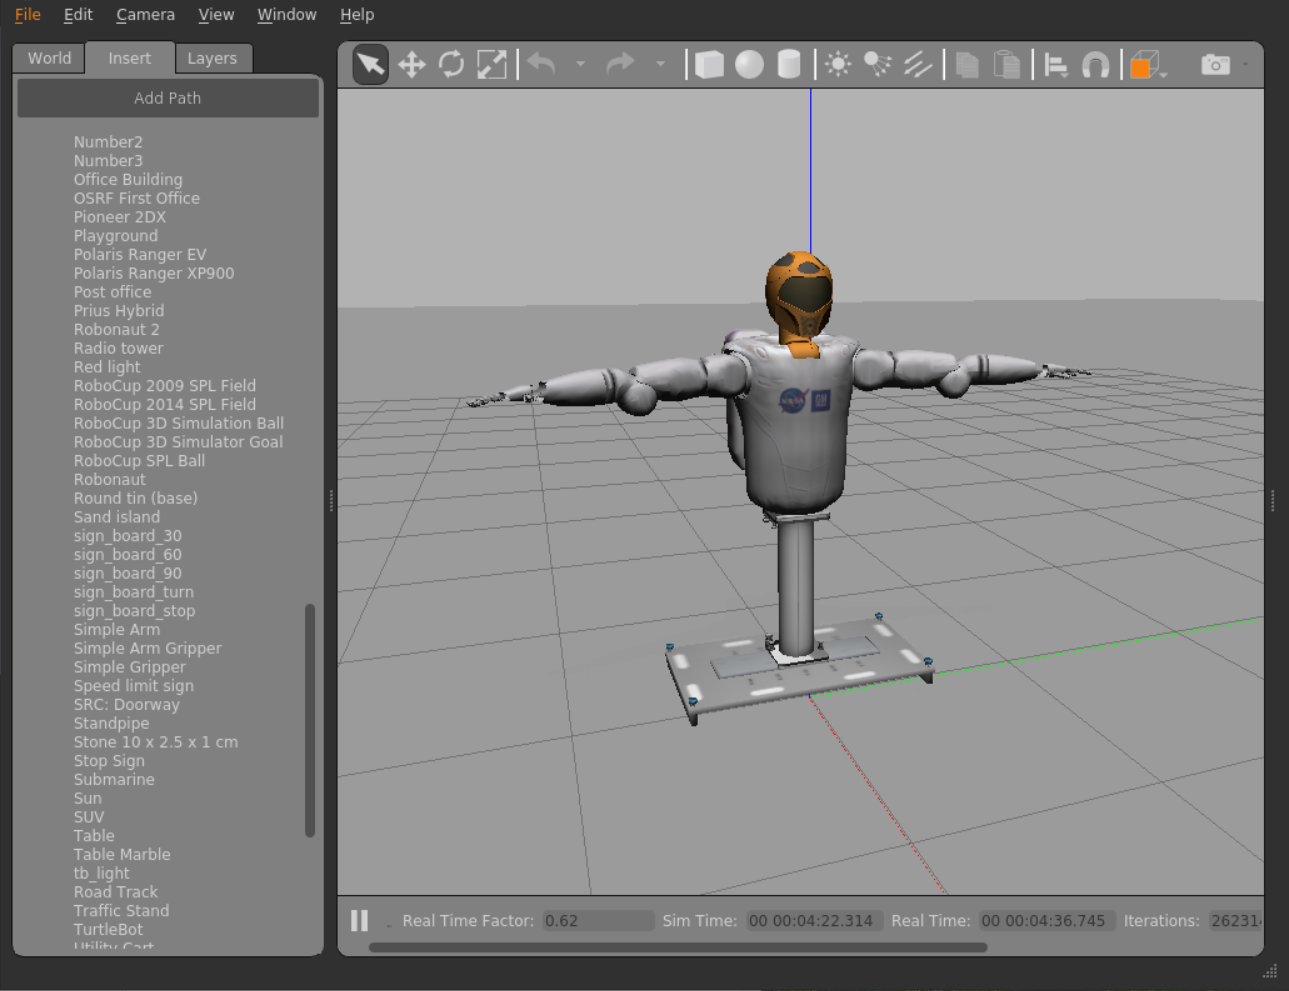
\includegraphics[width=0.5\textwidth]{figures/02marco_conceptual/Gazebo.PNG}
    \caption{\label{fig:ROS_gazebo} Robonauta 2 de la NASA simulado en Gazebo} 
    Fuente: \textit{Fabricación propia}
    \end{figure}

\subsubsection{RVIZ}
\textit{Robot Visualizer} o Rviz es una interfaz gráfica tridimensional de ROS que permite observar datos, mensajes, estados en tiempo real y otros elementos, de lo que cree el robot que está ocurriendo. El simulador permite la integración con la información recibida por los diversos paradigmas de ROS descritos anteriormente, como también es posible su integración con la información provista por Gazebo, lo que permite testear los algoritmos utilizando tanto Gazebo si no se tiene acceso al robot físico o también utilizando el robot real \cite{kam_rviz_2015}. Se puede observar en la Figura \ref{fig:ROS_rviz} en la sección central como Rviz presenta el mapa generado por el robot y en su extremo izquierda, la información provista por Gazebo mediante una cámara dispuesta en el robot.

\begin{figure}[h]
    \centering
    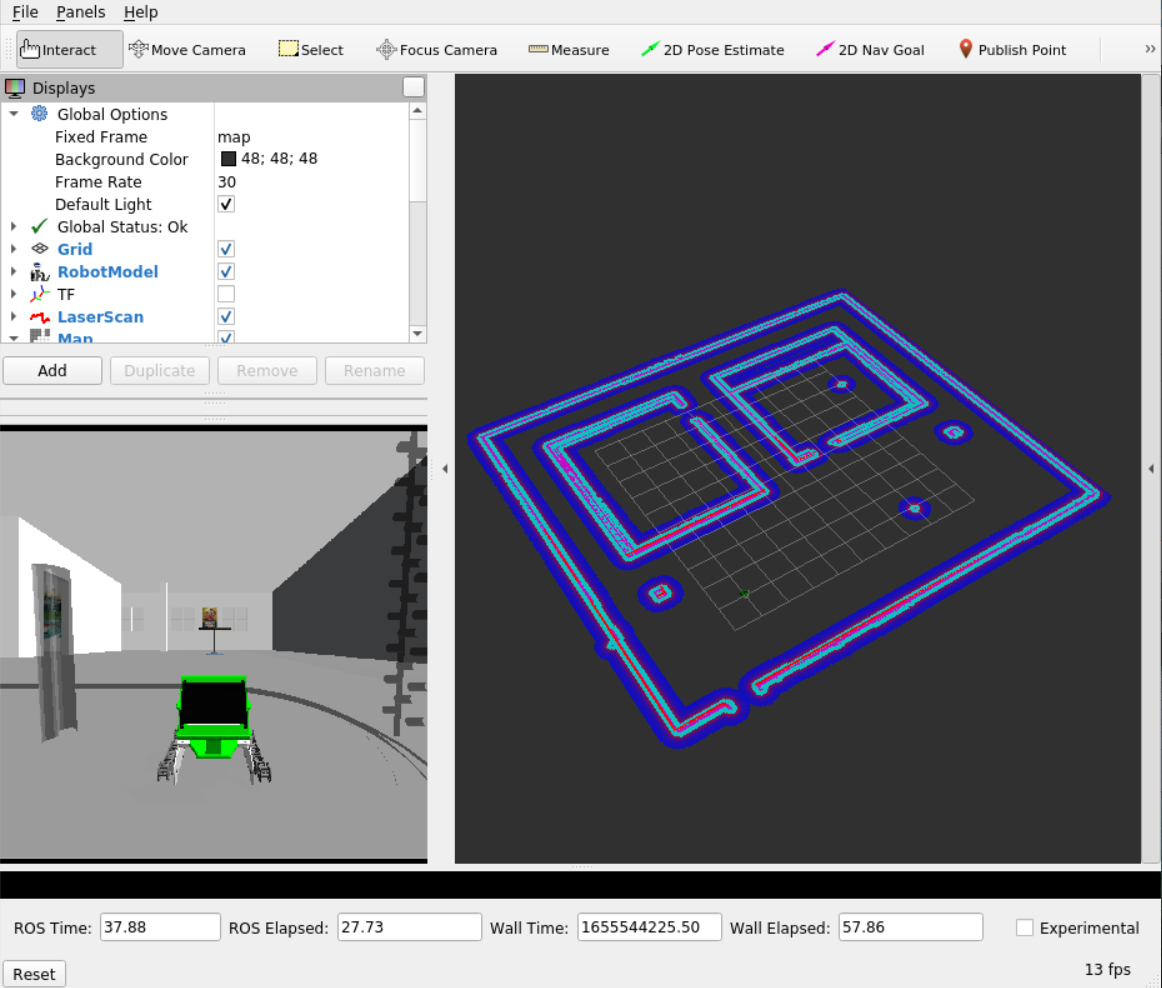
\includegraphics[width=0.5\textwidth]{figures/02marco_conceptual/Rviz.PNG}
    \caption{\label{fig:ROS_rviz} Visualización del entorno gráfico Rviz} 
    Fuente: \textit{Fabricación propia}
    \end{figure}
    
\newpage
\subsection{ALGORITMOS DE LOCALIZACIÓN}
La localización en el área de la robótica es la tarea de determinar en donde se encuentra el robot con respecto a su entorno. En el área de la robótica móvil es una de las tareas fundamentales a la hora de realizar un robot autónomo. En un escenario típico de localización se dispone del mapa del entorno y a través de la información recopilada por los sensores, el robot debe estimar su posición y orientación dentro del entorno \cite{huang_robot_2016}. Dentro de los algoritmos clásicos de localización utilizados en el estudio de la robótica móvil son los algoritmos \textit{Markov, Grid y Monte Carlo} los cuales se detallan en las siguientes secciones.


\textbf{ALGORITMO MARKOV}

El algoritmo Markov fue propuesto por primera vez en el año 1960 para el reconocimiento del habla, sin embargo, con el pasar de los años las aplicaciones del algoritmo se han expandido a diversas áreas, siendo una de esas la robótica \cite{reyes_mobile_2015}. Dicho algoritmo se basa en la información provista por los sensores y genera un modelo probabilístico de la localización del robot en su entorno y de esta manera el algoritmo entrega las posibles posiciones en donde el robot se puede encontrar. En el Algoritmo  \ref{alg:Algoritmo_Markov} se puede apreciar en detalle el funcionamiento del algoritmo.

\begin{algorithm}[H]
\centering
    \begin{algorithmic}[1]
        \Require $bel(x_{t1}), u_{t}, z_{t}, map$ 
        \vspace{1mm}
        \hline
        \vspace{1mm}
           \ForAll{$x_t$}
            $\overline{bel} = $∫p(x_{t}|u_{t},x_{t-1},m) \cdot bel(x_{t-1}) \partial(x_{t-1})$
            \State $bel(x_{t}) = \eta \cdot p(z_{t}|x_{t}, m) \cdot $\overline{bel(x_{t})}$
           \EndFor
           
        \State \Return $bel(x_{t})$
        \vspace{1mm}
        \hline
        \vspace{1mm}
    \end{algorithmic}
\caption{Pseudocódigo algoritmo Markov}
Fuente: \cite{thrun_probabilistic_2005}
\label{alg:Algoritmo_Markov}
\end{algorithm}

Este se deriva a partir del algoritmo Bayesiano, es decir, se requiere una posición inicial ($Bel(x_{t1}$), la cual mientras más certera mejor será el desempeño del algoritmo, con la diferencia de que el algoritmo de Markov también requiere el mapa ($map$) del entorno. Luego por cada posición el algoritmo iterará para entregar el modelo probabilístico con respecto a la localización del robot. Autores como Rajesh Kannan han utilizado el algoritmo para realizar un control mediante comandos de voz \cite{megalingam_ros_2019} siguiendo la estructura anteriormente dicha.

\textbf{ALGORITMO GRID}

El algoritmo aproxima la posición utilizando un filtro de histograma sobre una descomposición en la posición espacial. La versión más básica mostrada en el Algoritmo \ref{alg:Algoritmo_Grid} consta de una división del entorno mediante grillas del mismo tamaño y de la probabilidad de que el robot se encuentre en dicha grilla mediante la información provista por los sensores, es esencial entregar al algoritmo el tamaño de las cuadrículas ya que un tamaño menor indica mayor precisión a cambio de un mayor tiempo de localización. También el algoritmo toma en cuenta el modelo del movimiento del robot \textit{motion\_model} y la información provista por los sensores mediante \textit{measurement\_model}. Una aproximación del algoritmo es implementado por Zengfeng Wang en \cite{wang_grid-based_2018}, en donde mediante la información provista por sensores inalámbricos se logra localizar en el entorno.

\begin{algorithm}[H]
\centering
    \begin{algorithmic}[1]
        \Require $\{p_{k,t-1}\}, u_{t}, z_{t}, m$ 
        \vspace{1mm}
        \hline
        \vspace{1mm}
           \ForAll{$k$}
           $\overline{p}_{k,t} = $ \sum_{i=0}^{n} p_{i,t-1} \textbf{motion\_model}(mean($x_{k}$), $u_{t}$,mean($x_{i}$)) 
            \State $p_{k,t} = \eta \cdot \overline{p}_{k,t}$ \textbf{measurement\_model}($z_{t}$, mean($x_{k}$), m))
            
           \EndFor
        \Return $\{p_{k,t}\}$
        \vspace{1mm}
        \hline
        \vspace{1mm}
    \end{algorithmic}
\caption{Pseudocódigo algoritmo Grid}
Fuente: \cite{thrun_probabilistic_2005}
\label{alg:Algoritmo_Grid}
\end{algorithm}


\textbf{ALGORITMO MONTE CARLO}

El MCL (Algoritmo Monte Carlo de Localización) es uno de los más populares e importantes entre los algoritmos de localización. Funciona a través de una probabilidad mediante partículas y se puede utilizar para la localización global y local \footnote{La localización global se utiliza al inicio, para encontrar la posición inicial del robot y la localización local se utiliza una vez que el robot empieza a moverse y se desea saber su posición durante el experimento.}. El modelo básico del MCL es un método no determinista utilizado para aproximar expresiones matemáticas complejas. Este método aplicado a la localización del robot se puede observar en el Algoritmo \ref{alg:Algoritmo_Monte_Carlo} en donde se encuentra la probabilidad de que el robot se encuentre en una posición mediante la información provista por sensores. El algoritmo se inicia con una serie de candidatos posibles de posición inicial y mediante nueva información provista por los sensores, el algoritmo determina la probabilidad de que el robot se encuentre en una determinada posición (las probabilidades bajas son eliminadas de la lista de posibles posiciones). Xiaoyu Wang muestra una posible implementación del algoritmo MCL modificado para la localización de un robot en un entorno controlado, realizando pruebas para la localización fija, mediante movimiento y el análisis de la localización una vez que el robot se mueve externamente de su posición
\cite{xiaoyu_adaptive_2018}.


\begin{algorithm}[H]
\centering
    \begin{algorithmic}[1]
        \Require $X_{t-1}, u_{t}, z_{t}, m$
        \vspace{1mm}
        \hline
        \vspace{1mm}
        \State $\overline{X}_{t} = X_{t} = \emptyset$
           \For{$m=1$ to $M$}
           \State $x_{t}^{[m]} =  $\textbf{ sample\_motion\_model}($u_{t}, x_{t-1}^{[m]} $)
           \State $w_{t}^{[m]} = $\textbf{ measurement\_model}($z_{t}, x_{t}^{[m]}, m $)
           \State $\overline{X}_{t} = \overline{X}_{t} + <x_{t}^{[m]}, w_{t}^{[m]}>$
           \EndFor
           \For{$m=1 $ to $M$}
           \State draw $i$ with probability \infty  $ w_{t}^{[i]}$
           \State add $w_{t}^{[i]}$ to $X_{t}$
           \EndFor
        \State \Return $X_{t}$
        \vspace{1mm}
        \hline
        \vspace{1mm}
    \end{algorithmic}
\caption{Pseudocódigo algoritmo Monte Carlo}
Fuente: \cite{thrun_probabilistic_2005}
\label{alg:Algoritmo_Monte_Carlo}
\end{algorithm}

\newpage
\subsection{ALGORITMOS DE MAPEO}
En la sección anterior se nombró que una de las tareas esenciales en la robótica móvil es la de localizarse en un entorno, ya que esto es clave para permitir la autonomía y lograr realizar las tareas asignadas, sin embargo, los algoritmos anteriormente descritos presentan un elemento en común, que es el parámetro del mapa. Un mapa construido adecuadamente es esencial para una correcta localización. La construcción del mapa supone crear una imagen 2D del entorno, de esta manera se visualizarán correctamente los objetos fijos como las murallas, objetos, estantes, entre otros. Existe una variación de un mapeo 3D planteado por Manuel González \cite{dos_reis_quantitative_2019}, en donde se observan las cualidades de generar un mapa tridimensional del entorno en donde se ubique el robot. El algoritmo más importante es el \textit{Grid Mapping} el cual es descrito en la siguiente sección y que dio pasos a otros algoritmos de mapeos como lo es el algoritmo \textit{Hector Mapping}, descrito a continuación. \footnote{Si bien existen otros importantes como GraphSLAM y FastSLAM, estos se detallarán en la sección de algoritmos SLAM debido a la utilización de dicha técnica.}

\textbf{ALGORITMO GRID MAPPING}

El algoritmo Grid Mapping es el algoritmo estrella entre los algoritmos de mapeos debido a la simpleza de su funcionamiento. Se basa en la probabilidad de que una celda esté ocupada o no según los datos que se reciben por parte de los sensores. El algoritmo básico se puede observar en el Algoritmo \ref{alg:Algoritmo Grid Mapping} en donde esencialmente se utiliza la información provista por los sensores para generar el mapa correspondiente. En caso que el sensor detecte un objeto, la casilla se marcara y en caso contrario se mantendrá desocupada \cite{sankalprajan_comparative_2020}. 

\begin{algorithm}[H]
\centering
    \begin{algorithmic}[1]
        \Require $\{l_{t-1},i\}, x_{t}, z_{t}$
        \vspace{1mm}
        \hline
        \vspace{1mm}
        \ForAll{cells $m_{i}$}
            \If{$m_{i}$ in perceptual field of $z_{i}$}
                \State $l_{t,i} = l_{t-1,i} $ + \textbf{inverse\_sensor\_model}($m_{i}, x_{t}, z_{t}$)
            \Else{$l_{t,i} = l_{t-1, i}$}
            \EndIf
        \EndFor
        \State \Return $\{l_{t,i}\}$
        \vspace{1mm}
        \hline
        \vspace{1mm}
    \end{algorithmic}
\caption{Pseudocódigo algoritmo GMapping}
Fuente: \cite{thrun_probabilistic_2005}
\label{alg:Algoritmo Grid Mapping}
\end{algorithm}

Un ejemplo visual del algoritmo se puede observar en la Figura \ref{fig:GMapping} en donde se observa a la izquierda el mapa real del entorno y a la derecha el mapa generado por el algoritmo.

\begin{figure}[H]
    \centering
    \begin{subfigure}[b]{0.40\textwidth}
    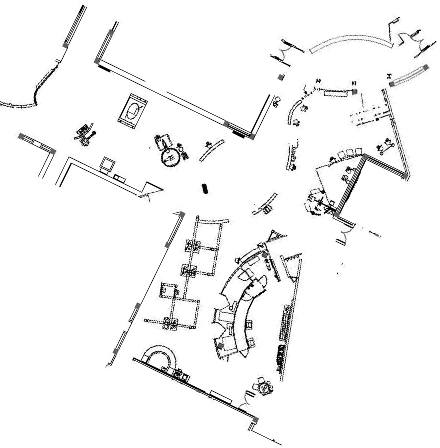
\includegraphics[width=\textwidth, height=\textwidth]{figures/02marco_conceptual/Mapa.PNG}
    \caption{Mapa del entorno}
    \label{fig:gmapping_sim}
    \end{subfigure}
    \begin{subfigure}[b]{0.40\textwidth}
    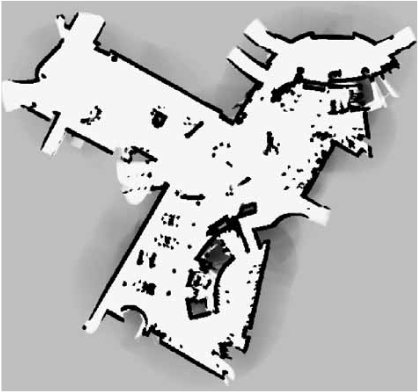
\includegraphics[width=\textwidth, height=\textwidth]{figures/02marco_conceptual/Mapa_generado.PNG}
    \caption{Mapa generado por GMapping}
    \label{fig:gmapping_map}
    \end{subfigure}
    \caption{Comparación entre el mapa real del entorno y el mapa generado por el algoritmo GMapping}
    Fuente: \cite{thrun_probabilistic_2005}
    \label{fig:GMapping}
\end{figure}

\textbf{ALGORITMO HECTOR MAPPING}

El algoritmo Hector Mapping, propuesto por Stefan Kohlbrecher y Oskar von Stryk en \cite{kohlbrecher_flexible_2011}, en donde se propone un algoritmo lo suficientemente preciso que tenga bajos requisitos tanto económicos, como computacionales. Al utilizar pocos recursos computacionales, dicho algoritmo es escalable a cualquier computador con procesadores de bajo peso y sobretodo, bajo consumo. Los resultados del mapeo utilizando el algoritmo sobre un ambiente simulado se pueden observar en la Figura \ref{fig:hector_slam_work}.

\begin{figure}[H]
    \centering
    \begin{subfigure}[b]{0.40\textwidth}
    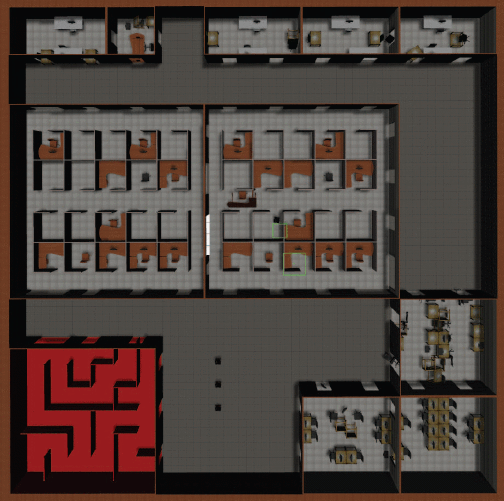
\includegraphics[width=\textwidth, height=\textwidth]{figures/02marco_conceptual/hector_slam_simulation.png}
    \caption{Ambiente simulado}
    \label{fig:hector_slam_sim}
    \end{subfigure}
    \begin{subfigure}[b]{0.40\textwidth}
    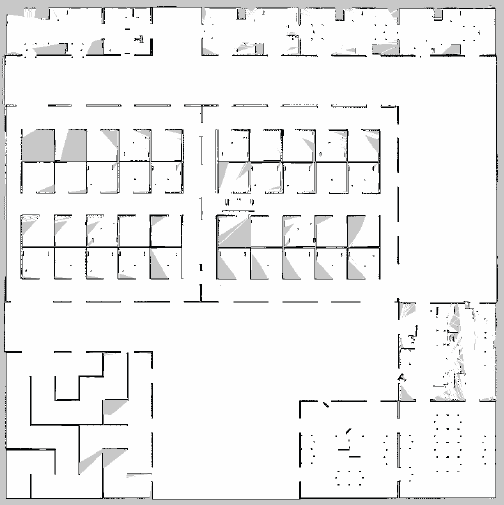
\includegraphics[width=\textwidth, height=\textwidth]{figures/02marco_conceptual/hector_slam_map.png}
    \caption{Mapa generado por Hector Mapping}
    \label{fig:hector_slam_map}
    \end{subfigure}
    \caption{Comparación entre el ambiente simulado y el mapa generado por el algoritmo Hector Mapping}
    Fuente: \cite{kohlbrecher_flexible_2011}
    \label{fig:hector_slam_work}
\end{figure}

Si bien existen variaciones del algoritmo Hector Mapping, ya que el gran beneficio del algoritmo es su capacidad de adaptarse a las distintas necesidades del sistema, el funcionamiento básico es el mismo en todos los casos y se puede observar en el Algoritmo \ref{alg:Algoritmo Hector Mapping}, en donde, al solo utilizar información del lidar se realiza la corrección del mapa. 

\begin{algorithm}[H]
\centering
    \begin{algorithmic}[1]
        \Require $HT_j, RT_J, Iter$
        
        \Ensure $TMatrix$
        \vspace{1mm}
        \hline
        \vspace{1mm}
        \State $MinResidual \leftarrow 1$

        \Function {MATCHFINDER}{$TransMx, HT_j, RT_j$}
            \While{$i<Iter$}
                \State $TMatrix \leftarrow$ ORIENICP($HT_j, RT_j$)
            \EndWhile
        \EndFunction
        
        \Function {ORIENICP}{$HT_j, RT_j$}
            \State $i \leftarrow 0$
            \State $HPoints \leftarrow HT_j$
            \State $RPoints \leftarrow RT_j$
            \State $MinResidual \leftarrow ICP(Hpoints, RPoints)$
            \If {$ORIENICP.Residual < MinResidual$} 
                \State $Trans \leftarrow ICP(Hpoints, RPoints)$
                \State $MinResidual \leftarrow OrienICP.Residual$
                \State \Return{$Trans$}
            \Else
                \State $PASS$
           \EndIf
        \EndFunction
        
        \Function {ALIGNORIENT}{$TransMX, Pose$}
            \State \hspace{4mm} $Pose[x,y].Rotate(TransMx)$
            \State \hspace{4mm} $Pose[x,y].Translate(TransMx)$
            
        \EndFunction
        \vspace{1mm}
        \hline
        \vspace{1mm}
    \end{algorithmic}
\caption{Pseudocódigo algoritmo Hector Mapping}
Fuente: \cite{kohlbrecher_flexible_2011}
\label{alg:Algoritmo Hector Mapping}
\end{algorithm}

\newpage
\subsection{ALGORITMOS DE NAVEGACIÓN}

Una vez que se ha construido el mapa y el robot se puede localizar en este, es necesario contar con algoritmos de navegación que permitan integrar la información provista por los algoritmos anteriormente señalados y así navegar por el entorno, es decir, a partir de la posición inicial y una posición final u objetivo, debe planificar la mejor ruta (esto puede ser en términos de eficiencia, costes, riesgos, entre otros) y realizar la ruta pertinente \cite{gul_comprehensive_2019}. El funcionamiento básico de un algoritmo de navegación debe en primera instancia dividir el mapa generado por los algoritmos de mapeo en cuadrículas \footnote{La división del mapa se puede realizar de manera discreta o de manera probabilística según se determine dentro del algoritmo} y determinar la ruta óptima como se observa en la Figura \ref{fig:ROS_navegacion}.

\begin{figure}[h]
    \centering
    \includegraphics[width=0.8\textwidth]{figures/02marco_conceptual/Navegación.PNG}
    \caption{\label{fig:ROS_navegacion} Cuadrícula de navegación} 
    Fuente: \cite{thrun_probabilistic_2005}
\end{figure}

Uno de los algoritmos clásicos de navegación y planeamiento de rutas es el A*, la versión básica del algoritmo que se puede observar en el Algoritmo \ref{alg:Algoritmo A*}. Consta de una cuadrícula o mapa, una posición inicial y una posición final, está diseñado de tal manera que si bien la solución encontrada no es la mejor, si es encontrada de manera rápida, por lo que se considera que la solución encontrada es un máximo óptimo. Existen variaciones como las identificadas en \cite{noauthor_global_nodate}, sin embargo, parte del algoritmo básico de la búsqueda A*.

\begin{algorithm}[H]
\centering
    \begin{algorithmic}[1]
        \Require $start, goal$
        \vspace{1mm}
        \hline
        \vspace{1mm}
        \State open\_list =  containing start
        \State  closed\_list = $\emptyset$
        \State  start.g = 0
        \State start.f = start.g + heuristic(start,goal)
        \While{ current is not goal}
            \State current = open\_list element with lowest f cost
            \State remove current from open\_list
            \State add current to closed\_list
            \ForAll{neighbor of current}
                \If{neighbor not in closed\_list}
                    \State neighbor.f = current.g + heuristic(neighbor, goal)
                    \If{neighbor is not in open\_list}
                        \State add neighbor to open\_list
                    \Else
                        \State openneighbor = neighbor in open\_list
                        \If{neighbor.g < openneighbor.g}
                            \State openneighbor.g = neighbor.g
                            \State openneighbor.parent = neighbor.parent
                        \EndIf
                    \EndIf
                \EndIf
                \If{$open\_list$ $is$ $\emptyset$}
                    \State \Return $false$
                \EndIf
                \State \Return{backtrack\_path(goal)}
            \EndFor
        \EndWhile
        \vspace{1mm}
    \hline
    \vspace{1mm}
    \end{algorithmic}
\caption{Pseudocódigo algoritmo A*}
Fuente: \cite{candra_application_2021}
\label{alg:Algoritmo A*}
\end{algorithm}

\newpage
\subsection{ESTADO DEL ARTE}

Las aplicaciones de la robótica móvil se dan en múltiples áreas, por ejemplo, en la exploración minera ayudando a extraer datos de la superficie, también se pueden dar en la exploración planetaria con los \textit{rovers} enviados a Marte. Operando en misiones de rescate y búsqueda de personas, reconocimiento de terreno, investigación militar, entre otros rubros más \cite{russell_artificial_2010}.

Es así como los robots móviles se definen como un \textit{``Un sistema electromecánico capaz de desplazarse de manera autónoma sin estar sujeto físicamente a un solo punto. Posee sensores que permiten monitorear a cada momento su posición relativa a su punto de origen y a su punto de destino. Normalmente su control es en lazo cerrado. Su desplazamiento es proporcionado mediante dispositivos de locomoción, tales como ruedas, patas, orugas, etc.''} \cite{sotelo_robots_2007}. 

En grandes rasgos los robots móvil se pueden identificar según el mecanismo que se utilice para realizar el movimiento, entre los cuales se destacan 3 grupos: Mediante ruedas, mediante extremidades y mediante orugas. Shigeo Hirose \cite{hirose_three_1991} describe como una primera aproximación la existencia de dichos grupos y los identifica de la siguiente manera:
\begin{itemize}
    \item \textbf{Aquellos robots que utilizan ruedas o una combinación de estas para desplazarse.} Si bien su implementación es más sencilla, están limitados por su adaptabilidad al terreno, sin embargo, son bastante eficientes en los terrenos parejos o con pequeñas elevaciones.
    \item \textbf{Aquellos robots que presentan piernas o extremidades para trasladarse.} Los robots que basan su movilidad en piernas, pueden adaptarse al entorno y este pasa a un segundo plano cuando se tienen altos grados de libertad, sin embargo, no son eficientes en términos energéticos, pero si les permiten mayor movilidad.
    \item \textbf{Aquellos robots que presentan articulaciones que les permiten reptar como las serpientes u otros reptiles para realizar el movimiento.} Este tipo de robots están compuestos por una serie de articulaciones independientes lo que les permite mayor facilidad de transporte. Usualmente tienen un cuerpo radial pequeño y largo, y el tamaño les permite adentrarse en entornos en que otros robots no pueden hacerlo.
\end{itemize}

Años más tarde, Farbod Fahimi \cite{fahimi_autonomous_2009} cataloga al primer grupo, es decir, a los robots que utilizan ruedas, en 2 nuevos grupos: los robots móviles \textit{hillary-type} y los \textit{car-like}. Por una parte los primeros se caracterizan por tener dos o más ruedas motrices independientes, mientras que por otra parte los segundos se caracterizan por tener un solo motor que alimenta a las ruedas y por ende el movimiento viene dado por un solo elemento.

Actualmente podemos encontrar robots en los hogares que facilitan la vida, como las aspiradoras roomba, robots que despachan pedidos en almacenes o incluso robots que en restaurantes van a dejar comida a la mesa, por lo que se estima que un porcentaje no menor de la población mundial tendrá contacto con robots dentro de la siguiente década. En esta línea se observa que los potenciales beneficiarios de un robot móvil es un grupo no menor de personas como lo pueden ser los dueños de casas, familias con adultos mayores, doctores y enfermeras en hospitales, restaurantes que deseen automatizar y agregar tecnología inteligente en sus dependencias e incluso almacenes que quieran innovar en tecnologías nuevas entre otros rubros más \cite{russell_artificial_2010}.

En esta línea, en conjunto con los avances de la robótica móvil, los algoritmos diseñados para contribuir con el área también deben avanzar a la par, es decir, con el paso de los años tanto algoritmos de mapeo, como de navegación y localización se han ido creando, mejorando y optimizando para crear robots más eficientes. En relación a esto, una técnica relativamente nueva y en donde los esfuerzos actuales se están centrando y por ende, nuevas líneas de investigación se están creando, es la técnica SLAM: \textit{Simultaneous Localization and Mapping} \cite{vSlam_takafumi_2017}. Es justamente el análisis a los algoritmos SLAM más utilizados en lo que se centrará la memoria.

\subsubsection{LOCALIZACIÓN Y MAPEO SIMULTÁNEOS}
La técnica SLAM utiliza de manera simultánea los algoritmos anteriormente descritos (los algoritmos de localización, navegación y mapeo) y como dice su nombre, el proceso de localización y mapeo se realizan de manera simultánea. Generalmente se utilizan cuando un robot se encuentra en un entorno desconocido en donde no se tiene información previa y este debe ubicarse dentro del entorno a partir de la información provista por los sensores durante el movimiento del robot y así generar un entorno virtual incremental \cite{grisetti_fast_2007}, esta problemática se puede observar en la Figura \ref{fig:problema_slam}. 

\begin{figure}[H]
    \centering
    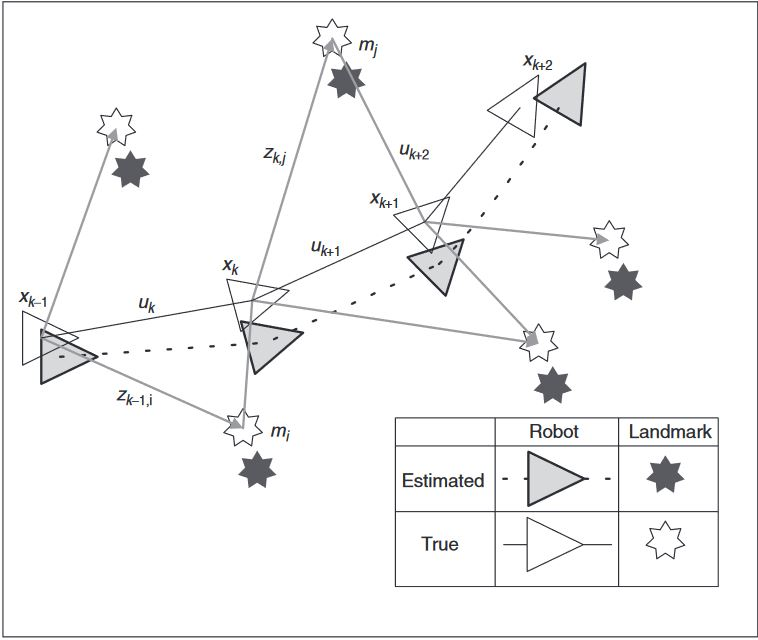
\includegraphics[width=0.5\textwidth]{figures/02marco_conceptual/slam_definicion.JPG}
    \caption{\label{fig:problema_slam} Problemática general del SLAM} 
    Fuente: \cite{durrant-whyte_simultaneous_2006}
\end{figure}

La aplicación de esta técnica es de suma importancia en entornos exteriores o no controlados, sin embargo, se siguen utilizando en la investigación en ambientes controlados por sus amplias capacidades. Es por ello, que la investigación de la técnica, la ha convertido en una de las más esenciales a la hora de construir un robot y estudiar el movimiento autónomo de estos.

Actualmente, se pueden identificar 3 grandes líneas de investigación (según de donde o como se obtenga la información para localizarse y producir el mapa) las que se pueden identificar como \textit{Laser SLAM}, \textit{Visual SLAM} o \textit{SLAM 3D} dependiendo de los sensores que se utilicen para obtener la información correspondiente. Si bien existen diversas ramificaciones de pseudo-algoritmos, el algoritmo básico planteado en el Algoritmo \ref{alg:Algoritmo SLAM}

\begin{algorithm}[H]
\centering
    \begin{algorithmic}[1]
        \Require $map\_size$
        \vspace{1mm}
        \hline
        \vspace{1mm}
        \State slam = init\_slam(map\_size)
        \For{n = 0; ;n+ +}
            \State image = acquire\_frame()
            \State predict(slam, robot\_model)
            \State j = 0
            \State lmk\_list = select\_lmks(slam)
            \State correl\_list = correl\_lmks(lmk\_list, frame)
            \For{i = 0, i < size(correl\_list) and j < nb\_correct; i++}
                \If{score(correl\_list[i]) > correl\_threshold}
                    \State correct\_slam(correl\_list[i])
                    \State j ++
                \EndIf
            \EndFor
            \State feature\_list = detect\_features(frame)
            \State j = 0
            \For{i = 0; i < size(feature\_list) and j < nb\_init; i++}
                \If{init\_lmk(feature\_list[i]}
                    \State j++
                \EndIf
            \EndFor
        \EndFor
        \vspace{1mm}
    \hline
    \vspace{1mm}
    \end{algorithmic}
\caption{Pseudocódigo algoritmo SLAM}
Fuente: \cite{vslam_2018}
\label{alg:Algoritmo SLAM}
\end{algorithm}

\begin{itemize}
    \item \textbf{\textit{Laser SLAM: }} También conocida como SLAM, corresponde a la técnica que utiliza láser o lidares para lograr el mapeo y la localización en un entorno. La noción de localización y mapeo de forma simultánea fue descrita inicialmente en 1986, pero no fue hasta la década del 2000 donde se logró implementar por primera vez en un automóvil autónomo.
    
    Los beneficios de utilizar láser como medio para obtener información es que son altamente confiables y el mapa creado no presentará errores acumulativos. Por otra lado, desde el punto de vista económico, existe una alta variedad de precios, por lo que la elección dependerá de los requisitos que se quieran satisfacer.
    
    \item \textbf{\textit{Visual SLAM: }} Técnica conocida como VSLAM corresponde a la utilización de cámaras (la única información que se tiene es la proveniente de las cámaras)  para generar una representación visual generando particiones visuales de lo observado y comparándolas con lo ya observado. Gracias a esta información se podrá tener más información sobre el entorno, sin embargo, la técnica está orientada a utilizarse en ambientes interiores debido a que la luz puede afectar y perjudicar el desempeño del algoritmo.
    
    El primer algoritmo en esta línea de investigación fue desarrollado el año 2003 llamado MonoSLAM, debido a que utilizaba una sola cámara monocular para obtener la información, cual tenía 6 grados de libertad \footnote{ Llámese grados de libertad a la cantidad de movimientos independiente que tiene una estructura, en un espacio tridimensional, el máximo son 6: 3 relacionados a la traslación y 3 relacionados a la rotación.}. Luego, tras los beneficios encontrados por las siguientes versiones del algoritmo, durante los años 2010 y 2016 se produjeron bastantes progresos con respecto a la técnica VSLAM \cite{4160954}.
    
    \item \textbf{\textit{SLAM 3D: }}  Por otra parte, esta nueva línea de investigación descrita por primera vez por Teng Hooi \cite{chan_lidar-based_2021}, en donde se realiza una aproximación tridimensional a la técnica SLAM agregando un ``grado de libertad" a los lidares (Esto se realizó utilizando lidares 3D \footnote{Un lidar 3D permite generar un mapeo tridimensional del entorno a través de una refracción interna del láser. }, en vez de las cámaras oculares), de esta manera el algoritmo puede generar un entorno tridimensional y navegar sobre él como se puede observar en la Figura \ref{fig:3D_SLAM} en donde en la parte superior se encuentra el entorno simulado y en la parte inferior la visualización 3D del entorno y la ruta de navegación realizada.
    
    Si bien existen diversos algoritmos relacionados con esta nueva línea de investigación, unos más complejos, otros con más variable y otros con más requerimientos, se puede encontrar un denominador común como lo es el algoritmo básico que se puede observar en el Algoritmo \ref{alg:Algoritmo 3DSLAM}.
\end{itemize}

\begin{figure}[H]
    \centering
    \begin{subfigure}[b]{0.45\textwidth}
    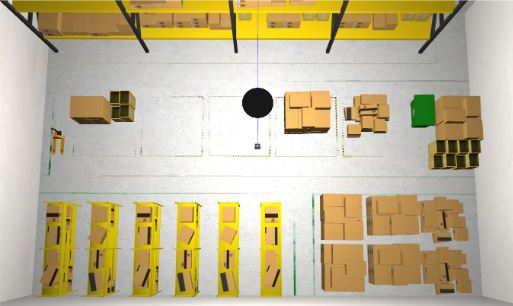
\includegraphics[width=\textwidth]{figures/02marco_conceptual/slam3d_1.JPG}
    \caption{Ambiente simulado}
    \label{fig:slam3d_1}
    \end{subfigure}
    \hspace{5mm}
    \begin{subfigure}[b]{0.45\textwidth}
    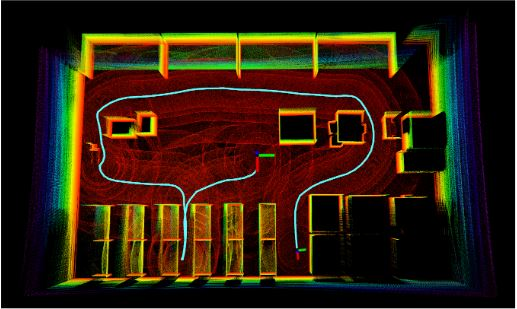
\includegraphics[width=\textwidth]{figures/02marco_conceptual/slam3d_2.JPG}
    \caption{Mapa generado por el algoritmo LIO-SAM}
    \label{fig:slam3d_2}
    \end{subfigure}
    \caption{ Reconstrucción tridimensional de un ambiente}
    Fuente: \cite{chan_lidar-based_2021}
    \label{fig:3D_SLAM}
\end{figure} 


\begin{algorithm}[H]
\centering
    \begin{algorithmic}[1]
        \Require $C$
        \Require $V_i$ points
        \Require $C_i$ plane
        \Require $S_c$
        \Require $N_i$
        \Require $\tau_\tau$
        \Require $\tau_m$
        \vspace{1mm}
        \hline
        \vspace{1mm}
        \State $C$ \leftarrow createGridCellStructure($S_c$)
        \ForAll{$v_i \in V$}
            \State writeToCorrespondingGridCell($v_{i}$, $C$)
        \EndFor
        \ForAll{$C_i \in C$}
            \State $C_i$ plane\leftarrow planarSegRansac($C_i$ points)
        \EndFor
        \While{$True$}
            \State $C_x \leftarrow getMinError(C)$
            \State $q \leftarrow merge(q, C_x)$
            \State $q \leftarrow growRegionGBS(q, C)$
            \While{ $q \neq \emptyset$}
                \State $q \leftarrow growRegionGBS(q, C)$
            \EndWhile
        \EndWhile
        \vspace{1mm}
    \hline
    \vspace{1mm}
    \end{algorithmic}
\caption{Pseudocódigo general para algoritmo 3D SLAM }
Fuente: \cite{3dslam_2018}
\label{alg:Algoritmo 3DSLAM}
\end{algorithm}

El problema de localización ha sido la piedra angular en la construcción de robots desde la década de los 50, dicho problema se puede entender como la tarea de que el robot estime la posición en un ambiente conocido a través de diversos sensores, sin embargo, un robot totalmente inteligente debe ser capaz de explorar los ambientes desconocidos donde la posibilidad de obtener tener un mapa del entorno está limitada o es inaccesible \cite{taheri_slam_2021}. En ambientes exteriores, uno de los elementos que se utiliza para la estimación de la posición es el \textit{Global Positioning System} o GPS, sin embargo, dicho sensor no es utilizable en un robot que se utilice en ambientes \textit{indoor}, por lo que se requerían nuevos sistemas y algoritmos para proveer y generar un mapa del entorno a la vez que se realiza una estimación de la posición, es bajo esta problemática que los algoritmos SLAM son creados, es decir, los algoritmos SLAM fueron creados para darle solución a los escenarios donde no se tiene referencia del mapa previamente \cite{thrun_probabilistic_2005}.

Durante los últimos 25 años, investigaciones y experimentos con algoritmos SLAM han llevado a la técnica a ser una de las más estudiadas y utilizadas en los robots modernos tanto para ambientes de interior como también para ambientes de exterior, llevando incluso los límites más allá de las fronteras iniciales y aplicándolos a ambientes aéreos, acuáticos, subterráneos, entre otros debido a los múltiples beneficios encontrados. En este tiempo, los algoritmos SLAM diseñados utilizan una seria de sensores como lo son las cámaras \textit{Red, Green and Blue} o RGB, sensores ultrasónicos, LIDARES, entre otros para estimar la posición en ambientes bidimensionales o tridimensionales \cite{li_topology_2016}. Si bien en dicho documento, se establece que el SLAM 2D es un problema que ya está resuelto, sin embargo, la creación de nuevas tecnologías, nuevos técnicas y requerimientos han reabierto el problema, debido a que la precisión, la velocidad y los nuevos datos que se generan por el avance de la tecnologías implicaban nuevas mejoras a los algoritmos creados con anterioridad \cite{taheri_slam_2021}.

En el año 2007, se aborda la problemática, sin embargo, se plantea desde otro punto de vista en el cual, esta vez se considera que el mapeo y la localización son tareas paralelas \cite{klein_parallel_2007}, no fue hasta esta investigación en donde los algoritmos SLAM fueron conocidos. Además de dar una primera noción sobre una posible solución a la localización y mapeo de manera simultánea, en dicho paper se establecen las implicancias de tener un mapa adecuado las cuales se pueden resumir en los siguientes 3 puntos:
\begin{enumerate}
    \item En primer lugar, los mapas son necesarios para poder realizar la planificación de rutas, evitar obstáculos, establecer puntos de interés, entre otros elementos. 
    \item En segundo lugar, bastantes aplicaciones de robots son justamente creadas para la construcción de mapas, por lo que se pueden encontrar robots cuyos objetivos son la construcción del mapa.
    \item Por último, que tan adecuada, eficiente, precisa y rápida es la localización del robot en el entorno depende significativamente de la precisión del mapa.
\end{enumerate}

Tal cual como se puede identificar en su nombre, los algoritmos SLAM presentan dos sub-algoritmos, algoritmos de localización y los algoritmos de mapeo \textit{(algoritmos de localización y mapeo simultáneos)}, los cuales inicialmente (década de los 50) se consideraban como elementos separados, sin embargo, las aproximaciones modernas, sobretodo aquellas que se han realizado en la última década, han mostrado que estos dos sub-algoritmos dependen directamente uno del otro, por lo que se podrían considerar como una sola problemática, por una parte para realizar un mapeo correcto, se requiere una correcta localización, mientras que para localizarse correctamente, se requiere un mapa preciso, es por ello, que los algoritmos SLAM abordan la problemática de localización y mapeo de manera simultánea. 

Las técnicas utilizadas para estimar la posición y así resolver el problema de localización se pueden clasificar en 2 tipos según el enfoque que se tenga: enfoque probabilístico y enfoque no probabilístico, mientras que los primeros al utilizar la información de los sensores estiman en base a una probabilidad de donde está el robot, los segundos utilizan un enfoque de filtrado de partículas y filtrados de Kalman. Estos últimos, específicamente aquellos que utilizan el filtro de Kalman, poseen una gran ventaja a la hora de estimar la posición debido a que son simples de implementar, lo que conlleva a que sean los algoritmos predilectos a la hora de utilizarlos, sin embargo, existen dos grandes problemas: Por una parte, los algoritmos que implementan dicho filtro son susceptibles a los errores acumulativos en la estimación de la posición, por otra parte, estos algoritmos solo se pueden utilizar en sistemas lineales \footnote{La gran mayoría de los sistemas robóticos son no lineales, sin embargo, estos se pueden linealizar rápidamente utilizando herramientas creadas para utilizar el filtrado de Kalman como lo es el \textit{Extended Kalman Filter} o EFK.}. 

\begin{figure}[h]
    \centering
    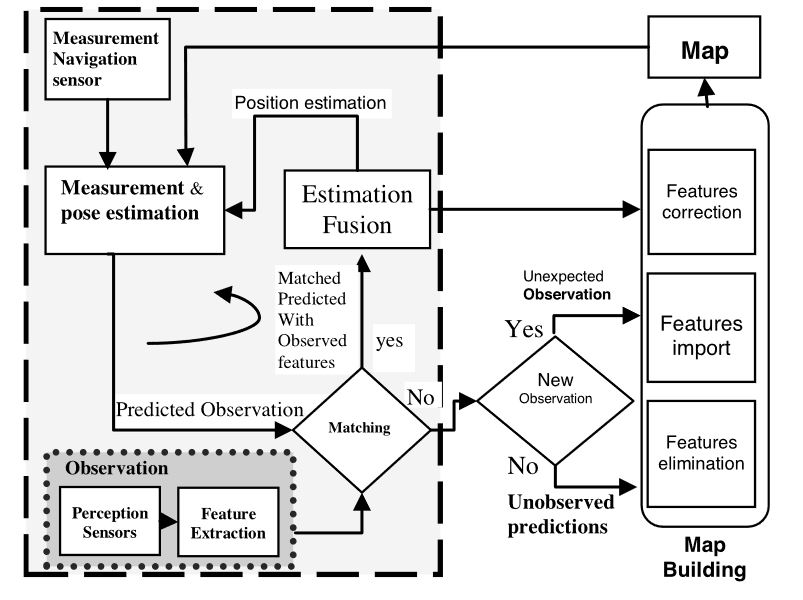
\includegraphics[width=0.8\textwidth]{figures/02marco_conceptual/esquema_general_slam.JPG}
    \caption{\label{fig:esquema_slam} Esquema general de los algoritmos SLAM} 
    Fuente: \cite{john_sonar_1992}
\end{figure}

Con el paso del tiempo y la optimización de las técnicas utilizando el filtrado EFK se obtuvieron mejores resultados, sin embargo, el modelo inicial se mantuvo intacto, el cual se puede observar en la figura \ref{fig:esquema_slam}. En términos prácticos se puede resumir en los siguientes 5 pasos: 
\begin{enumerate}
    \item A partir de los primeros datos recibidos por parte de los sensores, se construye una primera versión del mapa.
    \item Se estima una primera posición en este mapa inicial.
    \item A partir del movimiento del robot, tanto la localización como el mapa se van actualizando mediante marcadores.
    \item Se asocian los nuevos puntos de interés y se realiza una relación entre los marcadores antiguos y los nuevos para actualizar el mapa.
    \item Por cada iteración, se actualiza la ruta planificada por el algoritmo utilizando el mapa que se va generando y la información de los sensores, hasta que el robot llega a su objetivo.
\end{enumerate}

La arquitectura detrás del algoritmo SLAM se puede separa en 4 elementos esenciales, los cuales se encargan desde la obtención de los datos hasta la producción del mapa y la estimación de la posición. Estos 4 elementos, se pueden observar en la Figura \ref{fig:arquitectura_slam}. En detalle, cada elemento tiene sus tareas respectivas y sigue un flujo definido:
\begin{enumerate}
    \item \textbf{\textbf{Sensory input: }} Corresponde a todos los datos provenientes de los sensores, como lo son las imágenes, los datos del lidar, encoders, entre otros.
    \item \textbf{\textit{Front-End: }} En esta sección, el algoritmo toma los datos provenientes de la etapa anterior (los cuales están sin procesar), realiza la transformaciones respectivas como lo son la extracción de las características principales, asociación de datos, asociar datos entre otras funcionalidades y envía los datos a la siguiente sección.
    \item \textbf{\textbf{Back-End: }} En el Back-End, el algoritmo toma los datos enviados por el Front-End, realiza una optimización del modelo a través de un ajuste de parámetros y luego también define la posición y construye el mapa con dichos datos. A partir de estos valores, se ajustan los marcadores identificados y se le entrega un feedback al Front-End.
    \item \textbf{\textit{SLAM: }} En la última etapa, el algoritmo construye el mapa y realiza la estimación de la posición a partir de lo entregado por el Back-End.
\end{enumerate}

\begin{figure}[h]
    \centering
    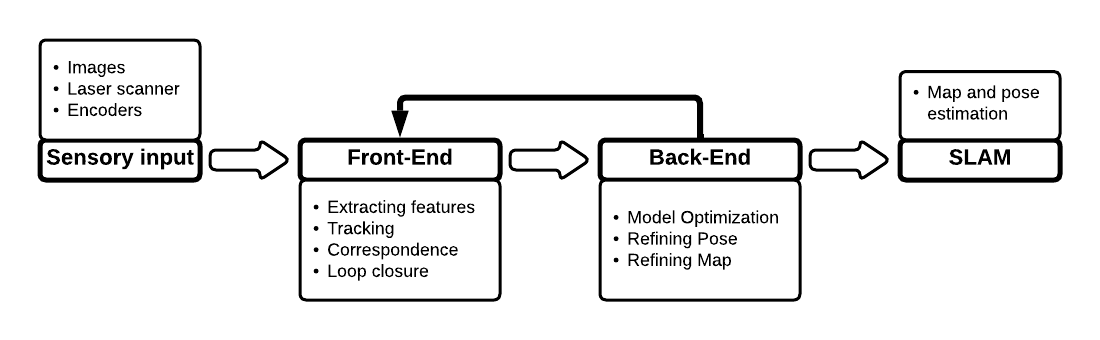
\includegraphics[width=0.8\textwidth]{figures/02marco_conceptual/arquitectura_slam.png}
    \caption{\label{fig:arquitectura_slam} Arquitectura algoritmo SLAM} 
    Fuente: \cite{taheri_slam_2021}
\end{figure}

\subsubsection{DIFICULTADES Y DESAFÍOS AL UTILIZAR SLAM}

Si bien existen una variedad de algoritmos SLAM, los autores concuerdas que por una parte el problema del SLAM es un problema en general, que aún no está resuelto y que existen 4 problemáticas en general: La asociación de los datos, La incertidumbre, el ruido o el error acumulativo y la complejidad temporal \cite{7482163}. Estas 4 problemáticas se definen a continuación: 

\begin{itemize}
    \item \textbf{La asociación de los datos: } Uno de los problemas claves a resolver en los algoritmos SLAM es la asociación de los datos, es decir, estimar correctamente los puntos y marcadores obtenidos por los sensores y asociarlos a nuevos datos. La asociación de datos permite al robot asociar el punto de origen, objetivo y la posición actual a coordenadas y referencias en el mapa \cite{problem_dissanayake_2011}.
    
    \item \textbf{La incertidumbre: } El problema de la incertidumbre hace alusión a la incerteza de los algoritmos (dado que se trabaja con algoritmos probabilísticos). En la literatura se pueden encontrar diversas definiciones de la problemática, sin embargo, se utilizará la definida en \cite{5136492}, en dónde se hace alusión a la capacidad del algoritmo de identificar las diversas rutas hacia un objetivo dependiendo de la posición en la que se encuentre. Este problema escala rápidamente en los ambientes reales en donde existen múltiples rutas para navegar desde un punto inicial hasta un punto final y existen obstáculos de diverso origen.
    
    \item \textbf{El ruido o el error acumulativo: } Los sensores cumplen un papel fundamental en los algoritmos SLAM debido a que la información para crear el mapa y localizarse proviene directamente de ellos. En la literatura se realiza un extenso estudio sobre la problemática \cite{bordoni_noise_1990} en donde se define como el ruido que tienen los sensores y por ende, el error asociado a la obtención de datos lo que termina provocando errores en el cálculo a la hora de estimar la ubicación y calcular los puntos de referencias.
    
    \item \textbf{La complejidad temporal: } Para evaluar el rendimiento de un algoritmo, se utiliza lo que comúnmente se conoce como complejidad temporal. En los algoritmos SLAM dicha complejidad se calcula aproximadamente en función de la cantidad de puntos utilizados para estimar la posición y los cálculos correspondientes para esta estimación. Dada la urgencia de tener algoritmos que funcionen en tiempo real, es un problema esencial en la literatura \cite{977154}. Actualmente existen una variedad de algoritmos que cumplen con diversos requisitos, donde se destaca el propuesto en \cite{4399179} con una complejidad computacional de $O(n)$, sin embargo, con un coste computacional bastante alto \footnote{Llámese coste computacional al coste asociado a los recursos consumidos por el algoritmo en cuestión.}.
\end{itemize}


















\newpage
\secnumbersection{PROPUESTA DE SOLUCIÓN}
En la presente sección se realiza una descripción detallada del algoritmo SLAM diseñado para cumplir los objetivos de la memoria, luego se presentará el diseño del algoritmo en conjunto con el pseudocódigo asociado y para finalizar un diagrama para identificar el flujo del mismo.


\subsection{DESCRIPCIÓN}
Tras lo escrito en la sección del marco conceptual y luego explayado en el estado del arte de los algoritmos SLAM, se pueden destacar 3 líneas de investigación de estos algoritmos en los cuales se pueden observar 4 problemas esenciales. En esta memoria se abordará una propuesta de solución para el problema de localización tridimensional en un robot móvil autónomo, es decir, el problema del SLAM 3D agregando un nuevo elemento en la asociación de los datos.

La propuesta del algoritmo SLAM, se basa fuertemente en la investigación realizada por Armin Hornung en \cite{hornung13auro}, en dónde se aborda la problemática desde un punto de vista nuevo y mediante un \textit{framework Open Source}. El framework utiliza la representación de volúmenes mediante octrees \footnote{ La representación volumétrica de octrees propuesta inicialmente en \cite{614315}, plantea la subdivisión recursiva del espacio tridimensional en octantes, creando un árbol con exactamente 8 subnodos y así sucesivamente.}, dicha representación se puede observar en la Figura \ref{fig:octree_tree}.

\begin{figure}[h]
    \centering
    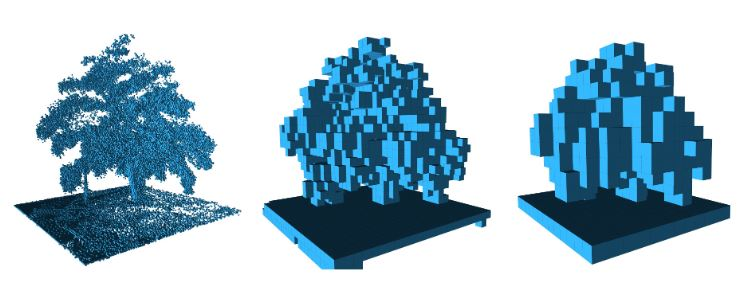
\includegraphics[width=0.8\textwidth]{figures/03propuesta_solucion/octree_mapping.JPG}
    \caption{\label{fig:octree_tree} Representación volumétrica utilizando octree de un árbol} 
    Fuente: \cite{inproceedings}
\end{figure}

EL trabajo desarrollado por Armin Hornung busca resolver el problema a partir de la utilización de LIDARES 3D para obtener dicha representación, lo que si bien aporta en reducir la incertidumbre de la posición, eleva en gran medida el coste económico asociado a dicha solución. Por lo que la propuesta expuesta y desarrollada en esta memoria utiliza la base matemática del algoritmo, sin embargo, se modifica para realizar el mapeo y localización tridimensional a través de una cámara de profundidad y un LIDAR bidimensional para realizar las correcciones necesarias a la información obtenida por la cámara, es decir, mejorar el asociamiento de los datos sin una aumentar en gran medida la incertidumbre del algoritmo a la hora de localizarse en el mapa y de esta manera, plantear un nuevo punto de acción a la problemática del SLAM 3D.

En términos generales, el algoritmo consta con 3 pasos:
\begin{itemize}
    \item Se debe inicializar el nodo maestro de ROS, de tal manera de enlazar correctamente los nodos hijos, establecer los tópicos de comunicación y los tipos de datos a enviar, como también se inicializan los nodos secundarios encargados del control del robot y obtención de datos de los sensores
    \item Se comienza con la obtención de los datos de los sensores, y a los marcadores obtenidos por la cámara se les realiza una corrección de manera que estos coincidan con los datos del LIDAR. Los datos una vez corregidos se guardan en un array multidimensional.
    \item El array multidimensional se procesa con el algoritmo octree recursivamente hasta el nivel 8 \footnote{ Se realizó una estimación del coste computacional asociado a cada nivel y la precisión del mapa generado y se obtuvo que el óptimo está entre el nivel 8 y el nivel 12. Cabe destacar que estos valores son \textbf{solo} para ambientes controlados o de interior.}. Para luego generar la estructura del mapa y transmitirlo en tiempo real.
\end{itemize}

La representación del mapa que el algoritmo genera, corresponde a una mapa probabilístico \footnote{Un mapa probabilístico asocia los datos a una probabilidad de que estén en el lugar indicado, en caso de que la probabilidad sea menor al filtro, entonces dicho dato se muestra como vacío.}. Un ejemplo de este mapa se puede observar en la Figura \ref{fig:mapeo_tridimensional}.

\begin{figure}[H]
    \centering
    \begin{subfigure}[b]{0.40\textwidth}
    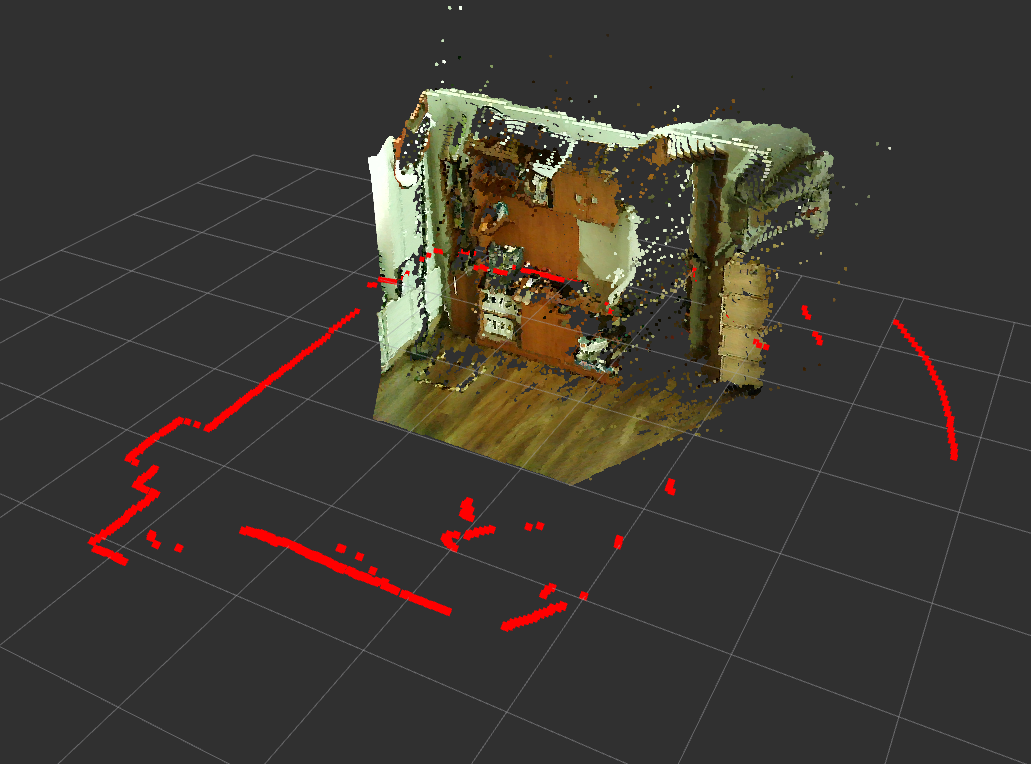
\includegraphics[width=5.5cm, height=4.9cm]{figures/03propuesta_solucion/slam_normal.png}
    \caption{Entorno mapeado utilizando la cámara de profundidad y LIDAR}
    \label{fig:gmapping_sim}
    \end{subfigure}
    \hspace{5mm}
    \begin{subfigure}[b]{0.40\textwidth}
        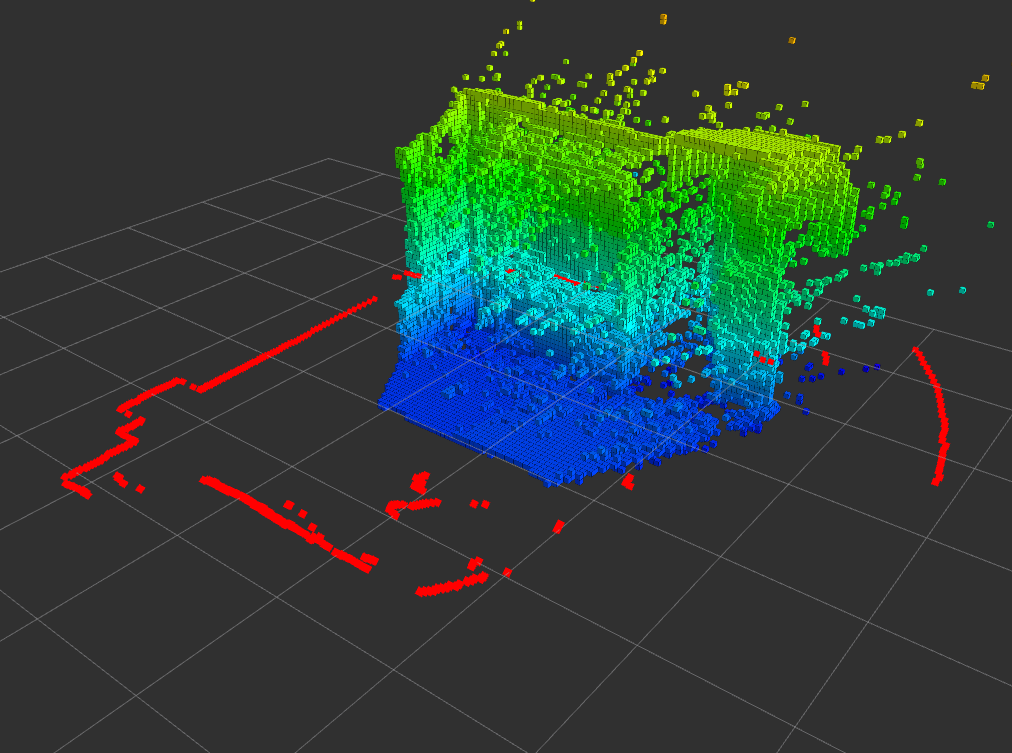
\includegraphics[width=5.5cm, height=4.9cm]{figures/03propuesta_solucion/slam_octree.png}
    \caption{Array multidimensional asociado a los datos obtenidos.}
    \label{fig:gmapping_map}
    \end{subfigure}
    \caption{Proceso de obtención de datos y generación del mapa tridimensional}
    Fuente: Fabricación propia
    \label{fig:mapeo_tridimensional}
\end{figure}


\newpage
\subsection{DISEÑO DEL ALGORITMO}

A continuación se muestra el pseudocódigo del algoritmo propuesto, el que se puede apreciar en el Algoritmo \ref{alg:Algoritmo 3DSLAM propuesto}. El algoritmo utiliza los datos de los diversos sensores para construir el mapa en dos dimensiones, el mapa tridimensional, obtener la orientación y localizarse dentro del mapa. Además se le debe entregar una resolución correspondiente y una precisión para la construcción tridimensional del mapa y finalmente una posición objetivo donde el robot debe ir.

\subsubsection{PSEUDOCÓDIGO}

\begin{algorithm}[H]
\centering
    \begin{algorithmic}[1]
        \Require $C_{d}$, $L_{d}$, $I_{d}$, $E_{d}$, data from sensors
        \Require $N = \{N_i, N_{i+1}, ...\}$, nodes for every sensor
        \Require $R$, resolution of the map
        \Require $A$, accuracy of the algorithm
        \Require $P_{f}$, final position
        \vspace{1mm}
        \hline
        \vspace{1mm}
        \State $A_{m}(R)$, $3DMap$, $2DMap  \leftarrow \emptyset$
        \State $P_a \leftarrow (0,0,0)$
        \ForAll{$N_i \in N$}
            \State initializeNode($N_i$)
        \EndFor
        \While{$Rospy \And P_a \neq P_f$}
            \State $P_{a} \leftarrow $ AMCL($3DMap$)
            \ForAll{$c_i \in C_d \And l_i \in L_d$}
                \State $2DMap  \leftarrow$ writeGridCell($l_{i}$, $2DMap$)
                \State $c_i \leftarrow$ correctionAlgorithm($c_i$, $l_i$) 
                \If {$c_i \notin A_{m}$} 
                    \State $A_{m} \leftarrow c_i$
               \EndIf
            \EndFor
            \State $3DMap \leftarrow$ octreeCodification($A_{m}, A$) 
            \State rvisualization($3DMap$, $2DMap$)
            \If{$P_a \neq P_f$}
                \State driveToGoal($3DMap$, $I_d$, $E_{d}$)
                \State updateStatusRobot()
            \Else
                \State \Return $GOAL$
            \EndIf
        \EndWhile
    \vspace{1mm}
    \hline
    \vspace{1mm}
    \end{algorithmic}
\caption{Pseudocódigo algoritmo 3D SLAM propuesto}
Fuente: Fabricación propia
\label{alg:Algoritmo 3DSLAM propuesto}
\end{algorithm}

\subsubsection{DIAGRAMA DE FLUJO DEL ALGORITMO}

A continuación se presenta el diagrama de flujo del algoritmo propuesto. En el diagrama, el cual se puede apreciar en la Figura \ref{fig:slam_3d_proposal_flujo}, se destacan 4 secciones definidas por 4 colores, cada una de estas secciones tiene tareas específicas las que se describen bajo el siguiente contexto: En color \textbf{verde} se indican los parámetros modificables, en color \textbf{naranjo} se demarcar los datos provenientes de los diversos sensores requeridos para el correcto funcionamiento del algoritmo, en color \textbf{morado} se indica el ciclo principal del algoritmo, es decir, el proceso de adquisición de datos, parametrización, filtrado y construcción del mapa y finalmente en \textbf{azul} el output del algoritmo el cual indica si se llegó al objetivo o no.

\begin{figure}[h]
    \centering
    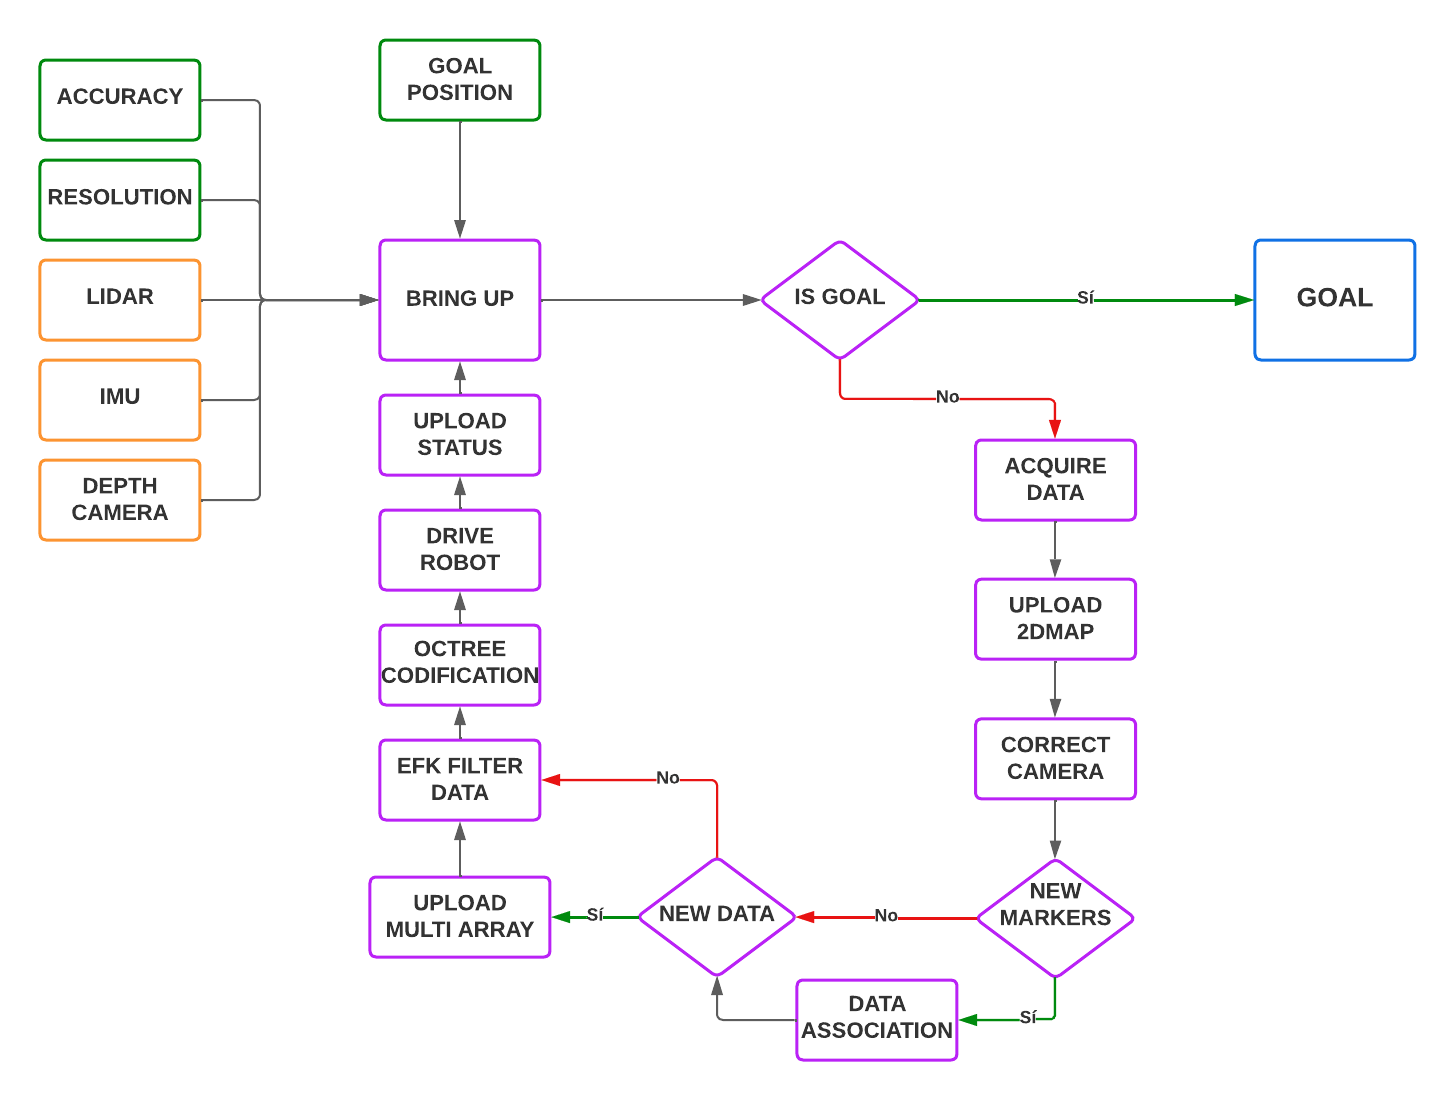
\includegraphics[width=0.8\textwidth]{figures/03propuesta_solucion/slam_3d_proposal.png}
    \caption{\label{fig:slam_3d_proposal_flujo} Diagrama de flujo del algoritmo propuesto} 
    Fuente: Fabricación propia
\end{figure}

Como se dijo anteriormente en el área central con color morado, se destaca el ciclo principal del algoritmo. En este, ocurre lo esencial para producir el SLAM 3D, es decir, se obtienen y procesan los datos provenientes de los sensores y los propios parámetros del algoritmo, se realiza la corrección de los datos de la cámara para que coincidan con los del LIDAR y se realiza un filtrado en los marcadores para diferenciar si el dato ingresado es nuevo o es un dato ya leído. Finalmente el algoritmo produce un filtrado EFK a los datos guardados en un array multidimensional para proceder con la codificación en octree, realizar el movimiento del robot y actualizar su status.




\begin{comment}

Se debe desarrollar la solución propuesta. Los subcapítulos por poner aquí son propios del autor. Se sugiere mencionar metodología usada. Es conveniente incorporar figuras y tablas para aclarar la solución, que deben indicar el número de la figura, su nombre y su autor o fuente (si las diseñas tú, la fuente es ``Elaboración propia''). Ver ejemplos en esta página y en la siguiente.

Cabe mencionar que aquí está la esencia del trabajo en lo que se refiere al aporte creativo del memorista, es el momento de demostrar que usted es un destacado profesional que creó, diseñó y/o llevó a cabo la solución propuesta.
\end{comment}
\newpage
\input{04diseño_experimental}
\newpage
\input{05experimentación}
\newpage
\secnumbersection{CONCLUSIONES}

\subsection{CONCLUSIONES GENERALES}
En los tiempos actuales donde la tecnología está abarcando nuevas áreas y la robótica se encuentra con nuevos desafíos, la creación de algoritmos que permitan a los robots entender, cuantificar e integrar los datos provenientes del entorno se hacen de suma importancia. El algoritmo propuesto propone además de implementar un mapeo tridimensional como bidimensional del entorno, una variable nueva a tomar en cuenta como lo son las zonas prohibidas, como también, abarca el problema de la asociación de los datos con la ayuda de dos sensores como lo son el LIDAR y una cámara de profundidad.

\subsubsection{RESULTADOS GENERALES}
Para validar el algoritmo creado, se utilizaron 5 ambientes físicos que simulan los distintos escenarios a los cuales un robot se puede enfrentar en el día a día. El ambiente uno simuló aquellos escenarios en dónde el robot se encuentra a campo abierto, el escenario dos simuló aquellos escenarios en dónde el robot se encuentra frente a un obstáculo, el ambiente tres simuló aquellos escenarios en dónde existen diversos obstáculos en el ambiente, por otro lado el ambiente cuatro simuló aquellos escenarios en donde el robot debe realizar una parada en su ruta y finalmente en el ambiente número cinco, el robot se vio enfrentado a la inclusión de zonas prohibidas en el mapa.

Dentro de las conclusiones más importantes obtenidas al momento de realizar la experimentación en los diversos ambientes, se pueden identificar las siguientes: 

\begin{itemize}
    \item Un modelo matemático del robot es esencial a la hora de implementar algoritmos de navegación, ya que la estimación de la posición dentro del mapa se basa fuertemente en estos cálculos. Pequeños errores en este cálculo pueden generar resultados desastrosos.
    \item El algoritmo propuesto presenta un mejor tiempo de generación del mapa que el algoritmo OctoMap, sin embargo, en promedio se demora el doble de tiempo en la generación del mapa en comparación con el algoritmo Hector. Esto se debe a que este último consiste únicamente en la generación de un mapa bidimensional, mientras que el algoritmo propuesto genera un mapa tridimensional y bidimensional a la vez.
    \item La precisión del mapa generado por el algoritmo propuesto está dentro de los estándares de la robótica mundial (sobre el 95\%), sin embargo, el algoritmo no está preparado para mapear ambientes exteriores debido a los problemas propios de los sensores utilizados y la precisión requerida debe ser sobre el 98\%.
    \item La implementación de detección de zonas prohibidas es una novedad en este tipo de algoritmos, ya que en ninguna investigación previa se encontró la implementación de este tipo de tecnología. 
    \item Se nota una diferencia no menor en el tamaño de los archivos entre un algoritmo de mapeo bidimensional y un algoritmo de mapeo tridimensional, sin embargo, esto hace sentido debido a las propias características de los mapas.
    \item El algoritmo propuesto tiene un consumo de memoria similar al algoritmo OctoMap en los ambientes 1, 2, 3 y 4, sin embargo, se nota una gran diferencia en el consumo de memoria en el ambiente 5. Esto debido a los propios cálculos que hace el algoritmo al momento de identificar las zonas prohibidas.
\end{itemize}

\subsubsection{LIMITACIONES}
La creación de un algoritmo SLAM 3D y la posterior implementación física de dicho algoritmo conlleva varias limitaciones entre las cuales se destacan el propio rendimiento delos sensores utilizados. Debido al aspecto económico, se adquirieron aquellos sensores que tenían el mejor rendimiento a bajo costo. Otras de las limitaciones que se identificaron a la hora de realizar la experimentación fueron las propias falencias electrónicas que debían resolverse al momento de ejecutar la memoria. Por último, también un a de las limitaciones más importantes fue el propio espacio físico de experimentación, en dónde el robot solo se pudo exponer a ambientes cerrados de aproximadamente 20 metros cuadrados.

\subsubsection{PRINCIPALES DESAFÍOS}
Dentro de los principales desafíos enfrentados durante el desarrollo de la memoria  se pueden destacar tres:
\begin{itemize}
    \item El primero desafío corresponde a los conocimientos mínimos para desarrollar la memoria. Dado que la memoria se centró en la robótica, varios conocimientos estaba fuera de los abarcados por los ramos dictados por la universidad por lo que fue necesario no solo realizar una gran lectura de papers y documentación de códigos, sino también el aprendizaje de nuevas tecnologías como lo son las herramientas de simulación y ROS.
    \item El segundo desafío corresponde a la implementación física del robot. Al momento de desarrollar la memoria, los algoritmos fueron testeados utilizando simuladores, en los cuales si bien se pueden simular físicas, el comportamiento electrónico y las propias falencias de los sensores no se pueden simular. Por lo que existió un cambio rotundo entre el comportamiento en la simulación del algoritmo y el comportamiento al momento de implementarlo en el robot físicamente.
    \item El tercer desafío hace alusión al ambiente número 5, específicamente a lo que corresponde con las zonas prohibidas. Inicialmente no se contempló la idea de zonas prohibidas en el algoritmo, por lo que fue un desafío implementar cambios en tiempo real del mapa generado que permitieran mostrar la zona prohibida.
\end{itemize}

\subsection{RESULTADOS PRINCIPALES}

\subsubsection{OBJETIVOS SECUNDARIOS}
\begin{itemize}
    \item Analizar los algoritmos de localización y navegación simultánea para adquirir los conocimientos del área a través de una investigación del estado del arte

    El estudio del estado del arte de los algoritmos de localización y navegación simultánea fue esencial para el desarrollo de la memoria. Este análisis se ve reflejado en la amplia bibliografía requerida para redactar la memoria y el contundente marco conceptual de la memoria. Por lo que el objetivo fue cumplido.
    
    \item Diseñar un algoritmo de localización y navegación simultánea tridimensional por medio de la utilización de una cámara de profundidad y un lidar para construir un mapa tridimensional de bajo costo

    Relacionado directamente con el objetivo específico o principal de la memoria, la creación de un algoritmo SLAM tridimensional se observa durante el desarrollo de la experimentación. En donde no solo se crea el mapa bidimensional de los 5 ambientes, sino también se genera el mapa tridimensional de este y se puede navegar utilizando dichos mapas de referencia. Durante el desarrollo de la memoria se utilizó una cámara de profundidad de bajo costo al igual que el lidar, lo que permite dar una solución al problema mediante sensores de bajo costo.

    
    \item Evaluar el desempeño del algoritmo propuesto por medio de la implementación física del robot considerando diversos ambientes de prueba

    El tercer objetivo corresponde a la implementación del algoritmo en un robot físico y su testeo en diversos ambientes, al igual que el objetivo anterior, el cumplimiento del objetivo se puede observar en el capítulo correspondiente a las experimentaciones realizadas. En dónde se detalla tanto el robot físico diseñado para la memoria, como también los resultados del mapeo hecho por el robot. Por otro lado, este mapeo se analizó y se evaluó en base a las 10 métricas identificadas de donde se concluyen los resultados generales descritos anteriormente.
\end{itemize}

\subsubsection{OBJETIVO ESPECÍFICO}
\begin{itemize}
    \item Crear un algoritmo de localización y navegación simultánea utilizando una cámara de profundidad y un lidar para un robot móvil autónomo en ambientes controlados

    El cumplimiento de los objetivos secundarios detallados anteriormente permiten dar por logrado el objetivo específico de la memoria, dado que se creó un algoritmo de localización y navegación tridimensional utilizando una cámara de profundidad y un lidar. 
    
\end{itemize}


\subsection{TRABAJO FUTURO}
Aquellos interesados que deseen continuar con la investigación sería interesante plantear nuevas mejoras y nuevos puntos de vista para abordar el problema de la navegación y localización simultánea en la robótica móvil, es por ello que a continuación se indican los lineamientos donde el autor considera esencial trabajar a futuro.

\subsubsection{ROS2}
Como fue explayado en el documento, el algoritmo se realizó en el framework ROS - Noetic. Sin embargo, se indicó en los foros que a partir del año 2025 este dejaría de tener soporte oficial, es por ello, que es de suma importancia realizar una migración del trabajo realizado a versiones posteriores como lo son ROS 2, la cual además estar mejor optimizada, presenta nuevas utilidades y nuevas funcionalidades.

\subsubsection{RENDIMIENTO}
Si bien los resultados obtenidos fueron prometedores, sería interesante plantear el algoritmo en entornos no controlados y observar el comportamiento de este y analizar los resultados de este en ambientes más complejos, ya que ambientes tan pequeños no permiten dar certeza de los resultados obtenidos. Por otra parte, actualmente el algoritmo tiene un alto consumo de memoria al momento de identificar las zonas prohibidas, por lo que sería interesante optimizar el algoritmo para disminuir dicho consumo de memoria y así el algoritmo estar disponible a más robots.

\subsubsection{MOVILIDAD TRIDIMENSIONAL}
Actualmente el algoritmo de navegación está pensado en utilizar esencialmente el mapa bidimensional, esto quiere decir, que el robot solo se puede mover en ambientes en donde no existen elevaciones, cambios de altura o no se puede implementar en robots que por ejemplo, puedan volar. Es por ello que se plantea la posibilidad de modificar el algoritmo a futuro para permitir la movilidad tridimensional y no solo tener en cuenta el espacio tridimensional como está construido actualmente.

\subsubsection{PERMISIBILIDAD}
Una de las novedades que el algoritmo tiene es la implementación y reconocimiento de zonas prohibidas. Estas zonas, tal cual como dice su nombre, son zonas en donde el robot no puede ingresar aunque no existe obstáculo alguno. Sería interesante dar un elemento de permitibilidad, es decir, si todas las rutas posibles se encuentras obstruidas, permitir al robot ingresar a la zona prohibida para continuar con la tarea asignada.

\newpage
\secnumberlesssection{ANEXOS}

\begin{comment}

\textbf{PREPARACIÓN DEL AMBIENTE DE LA MEMORIA}

\begin{verbatim}
    sudo sh -c 'echo "deb http://packages.ros.org/ros/ubuntu 
    $(lsb_release -sc) main" > /etc/apt/sources.list.d/ros-latest.list'
\end{verbatim}

\begin{verbatim}
    sudo apt install curl # if you haven't already installed curl
    curl -s https://raw.githubusercontent.com/ros/rosdistro/master/ros.asc 
    | sudo apt-key add -
\end{verbatim}

\begin{verbatim}
    sudo apt update
\end{verbatim}

\begin{verbatim}
    sudo apt install ros-noetic-desktop-full
\end{verbatim}

\begin{verbatim}
    echo "source /opt/ros/noetic/setup.bash" >> ~/.bashrc
    source ~/.bashrc
\end{verbatim}

\begin{verbatim}
    sudo apt install python3-rosdep python3-rosinstall 
    python3-rosinstall-generator python3-wstool build-essential
\end{verbatim}

\begin{verbatim}
    sudo apt install python3-rosdep
\end{verbatim}

\begin{verbatim}
    sudo rosdep init
    rosdep update
\end{verbatim}

\newpage
\textbf{SECCIÓN DE CÓDIGOS DEL TIPO LAUNCH FILE}

\textbf{ros\_serial.launch}
\begin{verbatim}
<launch>
    <node 
        pkg="rosserial_python" 
        name="arduino_node" 
        type="serial_node.py">
        <param 
            name="port" 
            value="/dev/ttyACM0" 
        />
        <param 
            name="baud" 
            value="115200" 
        />
    </node>
</launch>
\end{verbatim}

\textbf{ld19.launch}
\begin{verbatim}
<launch>
    <node 
        name="LD19" 
        pkg="ldlidar_stl_ros" 
        type="ldlidar_stl_ros_node">
        <param 
            name="product_name" 
            value="LDLiDAR_LD19"/>
        <param 
            name="topic_name" 
            value="scan"/>
        <param 
            name="port_name" 
            value ="/dev/ttyUSB0"/>
        <param 
            name="frame_id" 
            value="base_laser"/>
        <param 
            name="laser_scan_dir" 
            type="bool" 
            value="true"/>
        <param 
            name="enable_angle_crop_func" 
            type="bool" 
            value="false"/>
        <param 
            name="angle_crop_min" 
            type="double" 
            value="135.0"/>
        <param 
            name="angle_crop_max" 
            type="double" 
            value="225.0"/>
    </node>
    <node 
        name="base_to_laser" 
        pkg="tf" 
        type="static_transform_publisher"  
        args="0.0 0.0 0.18 4.71 0.0 0.0 base_link base_laser 50"/>
</launch>
\end{verbatim}

\textbf{gazebo.launch}
\begin{verbatim}
<launch>
    <arg 
        name="extra_gazebo_args" 
        default="--verbose"/>
    
    <arg 
        name="world_file" 
        default="$(
            find robocop_description)/
            worlds/
            simulation_world_00/
            simulation_world_00.world"/>
    
    <param 
        name="robot_description" 
        command="$(find xacro)/xacro 
        $(find robocop_description)/urdf/robocop.xacro"/>
    <node 
        name="spawn_urdf"
        pkg="gazebo_ros" 
        type="spawn_model" 
        args="-param robot_description -urdf -model robocop"/>
    <include 
        file="$(find gazebo_ros)/launch/empty_world.launch">
        <arg 
            name="world_name" 
            value="$(arg world_file)"/>
        <arg 
            name="paused" 
            value="false"/>
        <arg 
            name="use_sim_time" 
            value="true"/>
        <arg 
            name="gui" 
            value="true"/>
        <arg 
            name="headless" 
            value="false"/>
        <arg 
            name="debug" 
            value="false"/>
        <arg 
            name="extra_gazebo_args" 
            value="$(arg extra_gazebo_args)"/>
    </include>
</launch>
\end{verbatim}

\textbf{camera.launch}
\begin{verbatim}
<launch>
    <node 
        name="usb_cam" 
        pkg="usb_cam" 
        type="usb_cam_node">
        <param 
            name="video_device" 
            value="/dev/video2" />
        <param 
            name="image_width" 
            value="640"/>
        <param 
            name="image_height" 
            value="480"/>
        <param 
            name="pyxel_format" 
            value="yuvj420p"/>
        <param 
            name="image_format" 
            value="rgb8"/>
        <param 
            name="camera_frame_id" 
            value="usb_cam"/>
        <param 
            name="io_method" 
            value="mmap"/>
    </node>
    <node 
        name="image_view" 
        pkg="image_view" 
        type="image_view" 
        respawn="false">
        <remap 
            from="image" 
            to="usb_cam/image_raw"/>
        <param 
            name="autosize" 
            value="true"/>
    </node>
</launch>
\end{verbatim}

\textbf{robocop\_map.launch}
\begin{verbatim}
<launch>
    <include 
        file="$(find robocop_description)/launch/ld19.launch"/>
    <include 
        file="$(find robocop_description)/launch/mapping/display_map.launch"/>
    <include 
        file="$(find robocop_description)/launch/mapping/ps4.launch"/>
    <include 
        file="$(find robocop_description)/launch/mapping/hector_mapping.launch"/>
</launch>
\end{verbatim}

\textbf{ps4.launch}
\begin{verbatim}
<launch>
    <group ns="j1">
        <node 
            name="ds4_joystick" 
            pkg="joy" 
            type="joy_node">
                <param 
                    name="dev" 
                    value="/dev/input/js1" />
        </node>
    </group>
    <node 
        pkg="robocop_description" 
        name="ps4Controller"
        type="ps4Controller.py"/> 
    <node 
        pkg="rosserial_python" 
        name="arduino_node" 
        type="serial_node.py">
        <param 
            name="port" 
            value="/dev/ttyACM0" />
        <param 
            name="baud" 
            value="115200" />
    </node>
</launch>
\end{verbatim}

\textbf{hector\_mapping.launch}
\begin{verbatim}
<launch>
    <node 
        pkg="hector_mapping" 
        type="hector_mapping" 
        name="hector_mapping">
        <param 
            name="base_frame" 
            value="base_link" />
        <param 
            name="odom_frame"
            value="base_link" />
    </node>
</launch>
\end{verbatim}

\textbf{display\_map.launch}
\begin{verbatim}
<launch>
    <arg 
        name="model" 
        default="$(find robocop_description)/urdf/robocop.xacro"/>
    <arg 
        name="multi_robot_name" 
        default=""/>
    
    <param 
        name="robot_description" 
        command="$(find xacro)/xacro $(arg model)"/>
    <node 
        pkg="rviz" 
        type="rviz" name="rviz" 
        required="true" 
        args="-d $(find robocop_description)/launch/robocop.rviz"/>

    <node 
        pkg="robot_state_publisher" 
        type="robot_state_publisher" 
        name="robot_state_publisher">
        <param 
            name="publish_frequency" 
            type="double" 
            value="50.0"/>
        <param 
            name="tf_prefix" 
            value="$(arg multi_robot_name)"/>
    </node>
    <node 
        name="joint_state_publisher" 
        pkg="joint_state_publisher" 
        type="joint_state_publisher"/>
</launch>

\end{verbatim}

\textbf{robocop\_auto.launch}
\begin{verbatim}
<launch>
    <include 
        file="$(find robocop_description)/launch/ld19.launch"/>
    <include 
        file="$(find robocop_description)/launch/auto/display_auto.launch"/>
    <include 
        file="$(find robocop_description)/launch/ros_serial.launch"/>
</launch>

\end{verbatim}

\textbf{display\_auto.launch}
\begin{verbatim}
<launch>
    <arg 
        name="model"
        default="$(find robocop_description)/urdf/robocop.xacro"/>
    <arg 
        name="multi_robot_name" 
        default=""/>
    <param 
        name="robot_description"
        command="$(find xacro)/xacro $(arg model)"/>
    <node 
        pkg="rviz" type="rviz" 
        name="rviz" required="true" 
        args="-d $(find robocop_description)/launch/robocop.rviz"/>
    
    <node 
        pkg="robot_state_publisher" 
        type="robot_state_publisher" 
        name="robot_state_publisher">
        <param 
            name="publish_frequency" 
            type="double" 
            value="50.0" />
        <param 
            name="tf_prefix" 
            value="$(arg multi_robot_name)"/>
    </node>
    <node 
        name="joint_state_publisher" 
        pkg="joint_state_publisher" 
        type="joint_state_publisher"/>
    <node 
        name="map_server" 
        pkg="map_server" 
        type="map_server" 
        args="$(
            find robocop_description)/
            worlds/
            real_world_00/
            real_world_00.yaml" />
    <include 
        file="$(
            find robocop_description)/
            launch/
            auto/
            amcl_robocop.launch"/>
    
    <node 
        pkg="move_base" 
        type="move_base" 
        respawn="false"
        name="move_base" 
        output="screen">
        <param 
            name="base_local_planner" 
            value="dwa_local_planner/DWAPlannerROS" />
    <rosparam 
        file="$(
            find robocop_description)/
            codes/
            navigation_stack/
            costmap_common_params.yaml" 
        command="load" 
        ns="global_costmap" />
    <rosparam 
        file="$(
            find robocop_description)/
            codes/
            navigation_stack/
            costmap_common_params.yaml" 
        command="load" 
        ns="local_costmap" />
    <rosparam 
        file="$(
            find robocop_description)/
            codes/
            navigation_stack/
            local_costmap_params.yaml" 
        command="load" />
    <rosparam 
        file="$(
            find robocop_description)/
            codes/
            navigation_stack/
            global_costmap_params.yaml" 
        command="load" />
    <rosparam 
        file="$(
            find robocop_description)/
            codes/
            navigation_stack/
            move_base_params.yaml" 
        command="load" />
    <rosparam file="$(
        find robocop_description)/
        codes/
        navigation_stack/
        dwa_local_planner_params.yaml" 
        command="load" />
    </node>
</launch>


\end{verbatim}

\textbf{amcl\_robocop.launch}
\begin{verbatim}
<launch>
    <node 
        pkg="amcl"
        type="amcl" 
        name="amcl">
        <param 
            name="min_particles"             
            value="500"/>
        <param 
            name="max_particles"             
            value="3000"/>
        <param 
            name="kld_err"                   
            value="0.02"/>
        <param 
            name="update_min_d"              
            value="0.20"/>
        <param 
            name="update_min_a"              
            value="0.20"/>
        <param 
            name="resample_interval"         
            value="1"/>
        <param 
            name="transform_tolerance"      
            value="0.5"/>
        <param 
            name="recovery_alpha_slow"      
            value="0.00"/>
        <param
            name="recovery_alpha_fast"      
            value="0.00"/>
        <param 
            name="gui_publish_rate"          
            value="50.0"/>
        <param 
            name="laser_max_range"           
            value="8"/>
        <param 
            name="laser_min_range"           
            value="0.3"/>
        <param 
            name="laser_max_beams"          
            value="180"/>
        <param 
            name="laser_z_hit"               
            value="0.5"/>
        <param 
            name="laser_z_short"             
            value="0.05"/>
        <param 
            name="laser_z_max"              
            value="0.05"/>
        <param 
            name="laser_z_rand"              
            value="0.5"/>
        <param 
            name="laser_sigma_hit"           
            value="0.2"/>
        <param 
            name="laser_lambda_short"        
            value="0.1"/>
        <param 
            name="laser_likelihood_max_dist" 
            value="2.0"/>
        <param 
            name="laser_model_type"          
            value="likelihood_field"/>
        <param 
            name="odom_model_type"           
            value="diff"/>
        <param 
            name="odom_alpha1"               
            value="0.1"/>
        <param 
            name="odom_alpha2"              
            value="0.1"/>
        <param 
            name="odom_alpha3"               
            value="0.1"/>
        <param 
            name="odom_alpha4"              
            value="0.1"/>
        <param 
            name="odom_frame_id"             
            value="odom"/>
        <param 
            name="base_frame_id"             
            value="base_link"/>
        
        </node>
</launch>
\end{verbatim}

\newpage
\textbf{SECCIÓN DE CÓDIGOS PARA EL CONTROL}

\textbf{ps4Controller.py}
\begin{verbatim}
#!/usr/bin/env python

from sensor_msgs.msg import Joy
import sys, rospy
from geometry_msgs.msg import Twist

def chatter_callback(mensaje):
    joystick_izquierdo = (
        round(mensaje.axes[0],
        3), 
        round(mensaje.axes[1], 3)
        )
    joystick_derecho = (
        round(mensaje.axes[2], 
        3), 
        round(mensaje.axes[5], 3)
        )
    botones = (
        mensaje.buttons[1], 
        mensaje.buttons[2], 
        mensaje.buttons[3], 
        mensaje.buttons[0])

    # Publish data to cmd_vel topic
    publisherMotores = rospy.Publisher('/cmd_vel', Twist, queue_size=10)
    twist = Twist()
    twist.linear.x = joystick_izquierdo[1]
    twist.angular.z = joystick_derecho[0]
    publisherMotores.publish(twist)


def nodoPS4():
    nombreNodo = "nodo_ps4"
    idUnico = True
    rospy.init_node(nombreNodo, anonymous = idUnico)
 
    nombreTopico = "/j1/joy"
    tipoTopico = Joy 

    rospy.Subscriber(nombreTopico, tipoTopico, chatter_callback)
    rospy.spin()


if __name__ == "__main__":
    global arduino
    nodoPS4()
    
\end{verbatim}

\newpage
\textbf{SECCIÓN DE CÓDIGOS PARA LA CÁMARA}

\textbf{camera.py}
\begin{verbatim}
#!/usr/bin/env python

import cv2
import numpy as np
import time

# Create a VideoCapture object
cap = cv2.VideoCapture(2)

# Check if camera opened successfully
if (cap.isOpened()== False):
    print("Error opening video stream or file")

# Read until video is completed
while(cap.isOpened()):
    # Capture frame-by-frame
    ret, frame = cap.read()
    if ret == True:
        # Change the display size
        frame = cv2.resize(frame, (320, 640))
        # Display the resulting frame
        cv2.imshow('Frame',frame)

        # Press Q on keyboard to  exit
        if cv2.waitKey(25) & 0xFF == ord('q'):
            break

    # Break the loop
    else:
        break

# When everything done, release the video capture object
cap.release()
\end{verbatim}

\newpage
\textbf{SECCIÓN DE CÓDIGOS PARA LOS MOTORES}

\textbf{controller\_motor.ino}
\begin{verbatim}
// Se importan las librerías
#include <ros.h>
#include <AFMotor.h>

// Se importan los mensajes
#include <geometry_msgs/Twist.h>

// Variables globales de ROS
ros::NodeHandle nHandler;

// Se instancian las variables
float linearVelocity;
float angularVelocity;
float turnRightVel;
float turnLeftVel;

int forwardRight, forwardLeft, turnRight, turnLeft;
AF_DCMotor Motor1(3);
AF_DCMotor Motor2(4);

const byte encoder_rightA = 18;
const byte encoder_rightB = 19;
const byte encoder_leftA = 20;
const byte encoder_leftB = 21;

static long counter_right = 0;
static long counter_left = 0;
static long counter_right_old = 0;
static long counter_left_old = 0;

volatile bool fired_right, fired_left;
volatile bool up_right, up_left;

double x = 0;
double y = 0;
double theta = 0;

double rightVelocity = 0.0;
double leftVelocity = 0.0;

int long currentTime = 0;
int long previousTime = 0;

float map_float(
    float x, 
    float in_min, 
    float in_max, 
    float out_min, 
    float out_max) {
  return (x - in_min) * (out_max - out_min) / (in_max - in_min) + out_min;
}

void callback(const geometry_msgs::Twist& vel){
  linearVelocity = vel.linear.x;
  angularVelocity = vel.angular.z;

  int right_velocity = 150;
  int left_velocity = 150;
  if (linearVelocity>0.1){
    Motor1.run(FORWARD);
    Motor2.run(FORWARD);
    Motor1.setSpeed(right_velocity);
    Motor2.setSpeed(left_velocity);
  }
  if (linearVelocity<-0.1){
    Motor1.run(BACKWARD);
    Motor2.run(BACKWARD);
    Motor1.setSpeed(right_velocity);
    Motor2.setSpeed(left_velocity);
  }
  if (angularVelocity>0.1){
    Motor1.run(FORWARD);
    Motor2.run(BACKWARD);
    Motor1.setSpeed(right_velocity);
    Motor2.setSpeed(left_velocity);
  }
  if (angularVelocity<-0.1){
    Motor1.run(BACKWARD);
    Motor2.run(FORWARD);
    Motor1.setSpeed(right_velocity);
    Motor2.setSpeed(left_velocity);
  }
  if (abs(angularVelocity)<0.1 and abs(linearVelocity)<0.1){
    Motor1.setSpeed(0);
    Motor2.setSpeed(0);
  }

}

// Creación de los nodos de ROS
ros::Subscriber<geometry_msgs::Twist> nodo_vel("cmd_vel", callback);

// Variables para la odometría
double odom_x = 1.0;
double odom_y = 0.0;
double odom_thet = 1.57;
void setup(){
  // Se ajustan los nodos
  nHandler.getHardware()->setBaud(115200);
  nHandler.initNode();
  nHandler.subscribe(nodo_vel);

  // Se ajustan los motores
  Motor1.setSpeed(0);
  Motor2.setSpeed(0);
  Motor1.run(RELEASE);
  Motor2.run(RELEASE);


  Serial.begin(115200);
}

void loop(){ 
  nHandler.spinOnce();

}

\end{verbatim}

\end{comment}

\newpage
% Bibliografía estilo APA:
\bibliographystyle{apalike-es}
\bibliography{bibliografia}{}

\end{document}
